\documentclass[11pt,twoside]{article}
\usepackage{geometry}
\usepackage{enumerate}
\usepackage{latexsym,booktabs}
\usepackage{amsmath,amssymb}
\usepackage{graphicx}
\usepackage[singlespacing]{setspace}
\usepackage{longtable} % 处理长表格
\usepackage{hyperref} % 处理超链接
\usepackage{caption} % 图表标题格式
\usepackage{makecell}
\usepackage{multirow}
\usepackage{array}
\usepackage{caption}
\usepackage{url}
\usepackage{booktabs}
\usepackage{pgfplotstable}
\usepackage{siunitx}   
\usepackage{natbib}  
\usepackage{caption}
\captionsetup[figure]{justification=centering}
\usepackage{algorithm}
\usepackage[noend]{algpseudocode} 
\usepackage{float}
\usepackage{listings}
\usepackage{xcolor}
\lstset{
  basicstyle=\ttfamily\footnotesize,
  keywordstyle=\color{blue},
  commentstyle=\color{gray},
  stringstyle=\color{red},
  breaklines=true,
  numbers=left,
  numberstyle=\tiny\color{gray},
  frame=single,
  tabsize=4,
  language=Python,
  captionpos=b
}


\pgfplotsset{compat=1.18}

\geometry{a4paper,left=2cm,right=2.0cm, top=2cm, bottom=2.0cm}

\newtheorem{Definition}{Definition}
\newtheorem{Theorem}{Theorem}
\newtheorem{Lemma}{Lemma}
\newtheorem{Corollary}{Corollary}
\newtheorem{Proposition}{Proposition}
\newtheorem{Algorithm}{Algorithm}
\numberwithin{Theorem}{section}
\numberwithin{Definition}{section}
\numberwithin{Lemma}{section}
\numberwithin{Algorithm}{section}
\numberwithin{equation}{section}
\title{Olympic Medal Prediction under a Zero-Inflated Model: Quantitative Analysis of Socioeconomic Development and Demographic Factors}
\author{My Name}
\date{August 2025} 
\begin{document}

\pagestyle{empty}

% =============================================================================
% Title page
% =============================================================================
\begin{titlepage}
\vspace*{.5em}
\center
\textbf{\large{The School of Mathematics}} \\
\vspace*{1em}
\begin{figure}[!h]
\centering

\includegraphics[width=180pt]{CentredLogoCMYK.jpg}
\end{figure}
\vspace{2em}
\textbf{\Huge{Olympic Medal Prediction under a Zero-Inflated Model:}} \\
\textbf{\Huge{Quantitative Analysis of Socioeconomic}} \\
\textbf{\Huge{Development and Demographic Factors}} \\[2em]
\textbf{\LARGE{by}}\\
\vspace{2em}
\textbf{\LARGE{Zhenyang Zhou}}\\
\vspace{6.5em}
\Large{Dissertation Presented for the Degree of\\
MSc in Operational Research with Data Science}\\
\vspace{6.5em}
\Large{August 2025}\\ 
\vspace{3em}
\Large{Supervised by\\Dr Bruce Worton}
\vfill
\end{titlepage}

\cleardoublepage

% =============================================================================
% Abstract
% =============================================================================
\begin{center}
\Large{Abstract}
\end{center}

This dissertation examines how national economic scale, population size, human development, and the number of participating athletes influence the distribution of Olympic medals. Specifically, using a zero inflation negative binomial model, the analysis reveals marked inequalities: wealthier and more populous nations dominate medal standings, while smaller or less developed countries are disproportionately represented in the 'zero medal' category. In addition, the interaction between GDP and population underscores the combined influence of economic resources and demographic scale, while the number of athletes directly shapes the opportunity structure for medal acquisition. Although the Human Development Index exerts only a modest direct effect, its interaction with the number of athletes substantially enhances the efficiency of the medal, thus highlighting the indirect role of long-term human capital investment in athletic performance. Methodologically, the ZINB model effectively captures zero inflation and overdispersion of medal counts, while also illuminating the complex interplay of multiple structural determinants. In practical terms, these findings provide quantitative evidence for policymakers and Olympic committees, thereby facilitating more efficient resource allocation, optimization of delegation size, and underscoring the strategic importance of sustained investments in education, healthcare, and social welfare to strengthen athletic competitiveness. 

\clearpage

% =============================================================================
% Acknowledgments
% =============================================================================
\begin{center}
\Large{Acknowledgments}
\end{center}

With heartfelt gratitude, I extend my sincere thanks to all who supported and encouraged me during the completion of this dissertation.

First and foremost, I am deeply grateful to my supervisor, Dr. Bruce Worton, for his invaluable academic guidance. His comprehensive, meticulous, and rigorous supervision was of great help in shaping and improving this dissertation.

My sincere thanks go as well to our program director, Kit Daniel Searle, for his thoughtful efforts in organizing activities and for his constant attention to our learning, well-being, and career development, which proved immensely beneficial.

Finally, I am profoundly thankful to my family and to my friends and fellow students. Their love, support, and encouragement have been a strong source of strength and companionship, making this journey both possible and meaningful.

\clearpage

% =============================================================================
% Own Work Declaration
% =============================================================================
\begin{center}
\Large{Own Work Declaration}
\end{center}

I attest that I am the sole author of this thesis and that all the content within it is my originalwork, except for any instances where I have clearly indicated otherwise in the text.

\cleardoublepage

% =============================================================================
% Table of contents
% =============================================================================
\pagestyle{plain}
\setcounter{page}{1}
\pagenumbering{Roman}

\tableofcontents
\clearpage
\listoftables
\listoffigures
\cleardoublepage

\pagenumbering{arabic}
\setcounter{page}{1}

% =============================================================================
% Introduction
% =============================================================================
\section{Introduction}
\label{sec.intro}

\subsection{Background}
\label{subsec:background}

The Olympic Games, as the most influential global sporting event, have long been recognized as a microcosm of international politics, economics, and culture. The distribution of medals not only reflects athletic performance but also embodies national image, international standing, and societal institutions \cite{kaplanidou2010}. As global sports competition intensifies, scholarly and policy interest in Olympic medal prediction has grown significantly, extending well beyond the domain of sports statistics. 

Historically, research on medal prediction can be traced back to the mid-20th century, when studies relied primarily on linear regressions or descriptive observations, emphasizing the role of population size and economic power in determining medal counts \cite{johnson2004}. Since the early 21st century, methodological advances have led to the adoption of non-linear regressions, Poisson regression, Negative Binomial regression, and other count models, which better accommodate the discrete and over-dispersed nature of medal data \cite{scelles2020}. At the same time, research frameworks have expanded from simple “population–economy” models to more comprehensive approaches that incorporate sports investment, education, political institutions, historical traditions, and cultural factors \cite{forrest2010}.

Empirical evidence shows that economic and demographic size explain much of the variation in medal distribution. Major powers such as the United States, China, and Russia consistently dominate the medal table, mainly due to their vast populations and economic resources. However, numerous “outliers” exist. Sub-Saharan African countries, despite their demographic weight, often underperform in the medal standings, a phenomenon linked to inadequate government funding, weak institutional support, and insufficient sports infrastructure \cite{amusa2003}. By contrast, smaller nations with limited resources, such as Jamaica and Cuba, have excelled in athletics and boxing, suggesting that sports traditions and event specialization can partially offset demographic and economic disadvantages.

Regional disparities further complicate the picture. Western nations not only lead in total medals but also maintain balanced success across multiple disciplines. East Asian countries such as Japan, South Korea, and China display excellence in selected sports (e.g., gymnastics, archery, and weightlifting). In contrast, nations in Latin America and Africa often depend on a handful of specialized events to secure medals. These regional asymmetries reflect differences in resource allocation, institutional environments, and cultural traditions, highlighting the limitations of prediction models across diverse contexts.

The Olympic Games Tokyo 2020 present a unique case study shaped by the COVID-19 pandemic. The Games were postponed by one year and held under strict health protocols, introducing multidimensional disruptions: national training systems were curtailed, international preparation schedules disrupted, and athletes’ mental health strained by uncertainty and isolation \cite{preuss2021}. Furthermore, financial and logistical constraints led to reduced delegation sizes in several developing nations. These factors collectively created a “non-normal” environment that tested the resilience and adaptability of both athletes and predictive models.

In sum, Olympic medal prediction is not merely a statistical exercise but an interdisciplinary inquiry bridging economics, sociology, political science, and cultural studies. The Tokyo 2020 Games offer a critical opportunity to refine methodological approaches and to understand better the structural mechanisms shaping international sporting performance, with broader implications for sports policy, global competitiveness, and equity in international sport.


\subsection{Aim of the Dissertation}
\label{subsec:aim}

The primary objective of this dissertation is to provide a comprehensive and rigorous statistical analysis of the determinants of Olympic medal counts across countries, with a particular emphasis on addressing issues of data sparsity, heterogeneity, and robustness. To achieve this goal, the study adopts the Zero-Inflated Negative Binomial (ZINB) regression model, which is well-suited for over-dispersed count data with excessive zeros.  

First, the dissertation seeks to construct a baseline econometric model that captures the relationship between key socio-economic indicators (e.g., GDP, population, Human Development Index, and number of athletes) and Olympic medal performance. By employing ZINB regression, the study aims to account for both the probability of a country winning zero medals and the expected number of medals conditional on participation.  

Second, the dissertation investigates whether the estimated effects of socio-economic covariates are robust to alternative model specifications. This includes comparisons with standard count models such as Poisson and Negative Binomial regressions, as well as extensions incorporating interaction terms (e.g., GDP $\times$ Population, Athletes $\times$ HDI). These analyses ensure that the substantive conclusions are not unduly sensitive to modeling choices.  

Third, the study conducts sensitivity analyses to evaluate how results change when key predictors are redefined, excluded, or interacted, and when certain influential groups (e.g., large countries such as the United States, China, or Russia) are excluded from the dataset. Such robustness checks ensure that findings are not driven by a small number of dominant cases.  

Finally, beyond methodological contributions, the dissertation aims to provide substantive empirical insights into the determinants of Olympic success. The analysis seeks to clarify the relative importance of economic resources, demographic size, human development, and the number of athletes, as well as their potential interactions. These findings are expected to contribute not only to the literature on sports economics but also to broader discussions on international competitiveness and resource allocation in sports policy.  

Through these objectives, the dissertation seeks to establish both methodological rigor and substantive relevance, ensuring that the analysis of Olympic medal outcomes is both statistically robust and theoretically meaningful.



\subsection{Structure of the Dissertation}

This dissertation is organized into six chapters, each of which builds upon the previous one to provide a coherent progression from data collection and modeling to empirical findings, robustness checks, and concluding insights.

\textbf{Chapter 1: Introduction} outlines the research background, the aims of the study, and the overall structure of the dissertation. By situating Olympic medal prediction within the broader context of international sporting competition and national macro-level factors, this chapter establishes the rationale and significance of the research.  

\textbf{Chapter 2: Data Collection, Preprocessing and Exploration} describes the dependent and independent variables, the data sources, and the preprocessing steps. It further presents exploratory data analysis, including distributional characteristics, descriptive statistics, correlation analysis, and multicollinearity diagnostics.  

\textbf{Chapter 3: Modelling} introduces the econometric framework, focusing on the Zero-Inflated Negative Binomial (ZINB) model. It discusses model selection, variable definitions, estimation procedures, and software implementation, followed by model interpretation and diagnostic checks.  

\textbf{Chapter 4: Results and Analysis} constitutes the core of the dissertation. It reports the estimation outcomes of the ZINB model, including both the count and inflation components, and assesses model fit. Residual analysis is performed to identify over- and underperforming nations. In addition, case studies of high-performing countries and heterogeneity analyses across population size, GDP level, delegation size, and HDI groups are presented.  

\textbf{Chapter 5: Robustness and Sensitivity Analyses} evaluates the stability of the findings by comparing alternative model specifications, testing with different sets of covariates, and performing subsample robustness checks. Visualization of model fit and interaction effects is also provided.  

\textbf{Chapter 6: Conclusion} synthesizes the findings and reflects on their broader significance. It highlights the theoretical and practical contributions of the study, discusses policy implications, acknowledges limitations, and proposes directions for future research.  

In summary, the structure of the dissertation reflects a logical progression from contextual grounding and data preparation, through methodological development and empirical analysis, to robustness checks and theoretical reflection. This organization ensures both scientific rigor and practical applicability of the findings.


% =============================================================================
% Background
% =============================================================================
\section{Data Collection, Preprocessing and Exploration}
This chapter describes the data used and its sources, as well as the pre-processing methods. In addition, exploratory data analysis provides an initial understanding of the overall characteristics of the dataset and a preliminary explanation of the relationships between variables.
\label{sec:background}

\subsection{Data Collection}
This dissertation takes the 206 National Olympic Committees (NOCs) participating in the Olympic Games Tokyo 2020 as its research subjects \cite{IOC2025NOCs}. It should be noted that these 206 participating entities are not strictly equivalent to the 195 sovereign states among the United Nations member states. According to the definition of the International Olympic Committee (IOC), the participating entities are 'recognized National Olympic Committees', which include not only the member states of the UN, but also several territories with independent Olympic Committees \cite{IOC2024Charter}. The following sections will provide a detailed introduction to the independent and dependent variables of the main dataset and their sources.

\subsubsection{Dependent Variable}
The total number of Olympic medals is viewed by governments worldwide as an immediate quantitative indicator of national prestige. It not only reflects a country's economic strength but also influences the political dynamics among major powers \cite{allison2002}. Like most papers \cite{andreff2008}\cite{schlembach2020}, this dissertation defines the total number of medals as the dependent variable, whose value is equal to the sum of the number of gold, silver, and bronze medals.

\subsubsection{Independent Variables}
The number of medals a country wins at the Olympics is positively correlated with its total population \cite{Bernard2004}.  Populous countries (such as China) have a larger talent pool and, in theory, are more likely to win more medals than countries with very small populations, such as Luxembourg.  However, the International Olympic Committee implements a quota system for each event---for example, a maximum of three athletes per country in track-and-field events---which means that population growth beyond a certain threshold no longer translates linearly into medals.  Therefore, this dissertation controls for population size while further introducing the actual number of athletes participating from each country as a variable directly influencing the total medal count.

National wealth levels are also important predictors.  High-income countries can invest more funds in training facilities, coaching staff, and sports research, thus enhancing competitive performance \cite{debosscher2008}.  Therefore, this dissertation further introduces the gross domestic product (GDP, in current US dollars) as a proxy for economic strength.

To fully capture socio-economic development, the study also employs the Human Development Index (HDI) published by the United Nations Development Program.   HDI combines life expectancy, years of schooling and national income per capita, with values ranging from 0 to~1, where higher values indicate better development \cite{sharma2015}.  It has been shown to have significant explanatory power for Olympic medal tallies \cite{Halsey2009}.

\subsubsection{Data Sources}

The detailed explanation and source of the variables are shown in the table below. All data is for the year 2021.

\begin{table}[htbp]
\centering
\renewcommand{\arraystretch}{1.3} 
\caption*{Table 3: Variable descriptions and data sources}
\begin{tabular}{c|c|c|c}
\hline
\textbf{Category} & \textbf{Name} & \textbf{Explanation} & \textbf{Data source} \\
\hline
\raisebox{-0.3\height}{\begin{tabular}{@{}c@{}}Dependent\\Variable\end{tabular}} &
Total medals &
\begin{tabular}{@{}c@{}}Total of gold, silver and\\bronze medals\end{tabular} &
\begin{tabular}{@{}c@{}}International Olympic\\Committee \cite{ioc2020medals}\end{tabular} \\
\hline
\multirow{4}{*}{\begin{tabular}{@{}c@{}}Independent\\Variables\end{tabular}} &
Population &
\begin{tabular}{@{}c@{}}Mid-year resident\\population\end{tabular} &
World Bank\cite{worldbank2021population} \\
\cline{2-4}
& GDP &
\begin{tabular}{@{}c@{}}Gross domestic product\\(current US dollars)\end{tabular} &
World Bank\cite{worldbank2021gdp} \\
\cline{2-4}
& HDI &
\begin{tabular}{@{}c@{}}Human Development\\Index (0--1 scale)\end{tabular} &
\begin{tabular}{@{}c@{}}United Nations\\Development Programme\cite{undp2021hdi}\end{tabular} \\
\cline{2-4}
& Athletes &
\begin{tabular}{@{}c@{}}Number of participating\\athletes\end{tabular} &
\begin{tabular}{@{}c@{}}International Olympic\\Committee\cite{olympedia2020athletes}\end{tabular} \\
\hline
\end{tabular}
\end{table}


\subsection{Data Preprocessing}
The \path{totalmedals.xls} file contains the names of all participating teams in the Olympic Games Tokyo 2020, their corresponding NOC codes, the total number of medals, and their rankings. The \path{population.xls} and \path{GDP.xls} files provide population and GDP data, respectively, including country names and codes. The population data cover the period from 1960 to 2023, while the GDP data cover the period from 1960 to 2024. Since data for some countries in 2021 are missing, multiple years of data are retained to facilitate missing value imputation in subsequent sections. The \path{HDI.xls} file contains each country’s ISO Alpha-3 code and its corresponding Human Development Index (HDI) value. The \path{Athletes.xls} file records the names of participating teams in the Olympic Games Tokyo 2020, their corresponding NOC codes, and the total number of athletes for each team.

\subsubsection{Data Merge}
Since \path{population.xls}, \path{GDP.xls}, and \path{HDI.xls} use ISO Alpha-3 country codes, whereas \path{totalmedals.xls} and \path{Athletes.xls} use NOC codes, it is not possible to directly match data sets. Therefore, the team names in \path{totalmedals.xls} and \path{Athletes.xls} are mapped to the country names in \path{population.xls}, \path{GDP.xls}, and \path{HDI.xls}. For unmatched cases, manual mapping is applied, using the 206 Olympic-participating teams as the reference for matching.

Finally, the five datasets are merged into a unified dataset named \path{dataset1.xls}, with the following fields in order: \textbf{Code}, \textbf{Team}, \textbf{Totalmedals}, \textbf{Rank}, \textbf{GDP}, \textbf{Population}, \textbf{HDI}, and \textbf{Athletes}.

\subsubsection{Missing Value Handling}

In this dissertation, missing values are not retained as empty cells; instead, appropriate imputation methods are applied to ensure that every observation has a valid numerical value. The specific approaches are as follows:  
\begin{enumerate}
    \item \textbf{Cases with a missing value for a single year but complete data for adjacent years}: A linear interpolation method is used to estimate the missing value based on the preceding and subsequent years' data.
    \item \textbf{Cases with missing data for recent years but available historical data}: The most recent available value is used for imputation (forward-fill method), assuming that the indicator remains relatively stable in the short term.
    \item \textbf{Cases with no recorded data in the historical series}: Reference values are taken from countries (or regions) with similar economic size, geographical location, or socioeconomic characteristics, combined with relevant international statistical sources to make reasonable estimates.
\end{enumerate}
By adopting the above classification strategy, the loss of information caused by missing values is minimized, ensuring the completeness and comparability of the dataset.

\subsection{Exploratory Data Analysis}
American statistician John Tukey formally proposed exploratory data analysis (EDA) \cite{tukey1962}in the 1970s. It emphasises exploring raw data with as few prior assumptions as possible through visualisation and statistical summaries before modelling or hypothesis testing, in order to discover data structures, anomalies, patterns, and relationships between variables.

\subsubsection{Distribution Characteristics of Total Medal Counts}

In the exploratory analysis of the medal distribution at the Olympic Games Tokyo 2020, the participating \textit{National Olympic Committees} (NOCs) were first classified into two categories based on their total medal counts: ``zero-medal NOCs'' and ``non-zero-medal NOCs.'' The number and proportion of each category were then calculated to produce Figure~\ref{fig: Medal distribution at the Olympic Games Tokyo 2020}, which visually illustrates the distribution of zero- and non-zero-medal NOCs. Subsequently, the total medal count was treated as a numerical variable and analyzed using methods commonly applied to continuous data. This allowed the generation of a box plot, shown in Figure~\ref{fig: Box plot of Total medals at the Olympic Games Tokyo 2020}, to further examine the distribution shape, central tendency, and outlier patterns of medal counts across NOCs.

As shown in Figure~\ref{fig: Medal distribution at the Olympic Games Tokyo 2020}, among the 206 participating NOCs, 93 won at least one medal, accounting for approximately 45.15\%, while 113 did not win any medals, accounting for about 54.85\%. This result indicates that in this edition of the Games, more than half of the participating NOCs did not appear on the medal table, and there is a clear disparity in medal acquisition among NOCs. The relatively high proportion of zero-medal NOCs provides a basis for subsequent statistical modeling, suggesting that zero inflation should be considered to more accurately capture the structural characteristics of the medal distribution.

\begin{figure}[!ht]
\centering
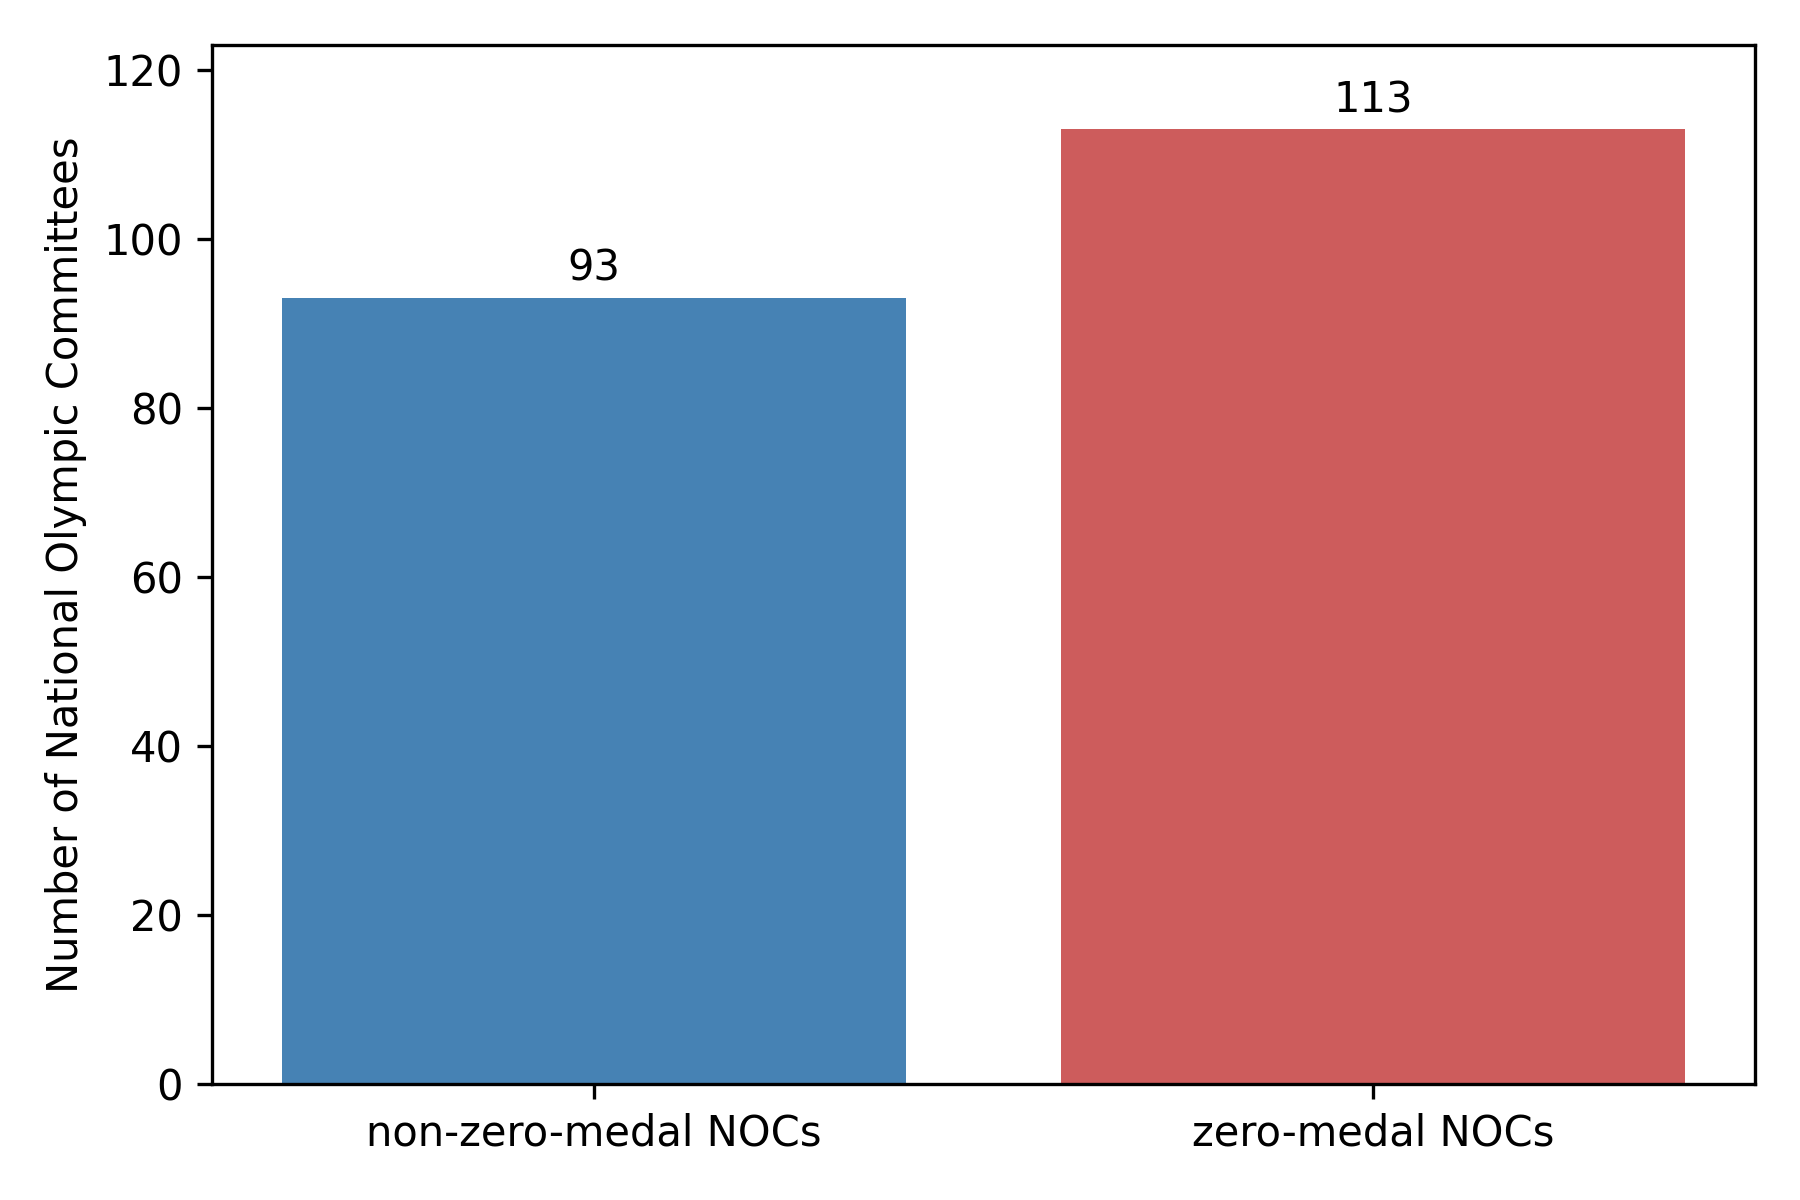
\includegraphics[width=0.8\textwidth]{zero_vs_nonzero_medals.png}
\caption{Medal distribution at the Olympic Games Tokyo 2020}
\label{fig: Medal distribution at the Olympic Games Tokyo 2020}
\end{figure}

Figure~\ref{fig: Box plot of Total medals at the Olympic Games Tokyo 2020} shows that the distribution of total medal counts is markedly right-skewed. Most NOCs have total medal counts concentrated within a low range, with a narrow interquartile range close to zero, indicating that the majority of NOCs won relatively few medals. Numerous outliers appear on the right-hand side, representing medal-dominant countries whose total counts are substantially higher than the rest, with extreme values exceeding 100 medals. This pattern highlights the concentration of Olympic medal resources among a few nations.

\begin{figure}[!ht]
\centering
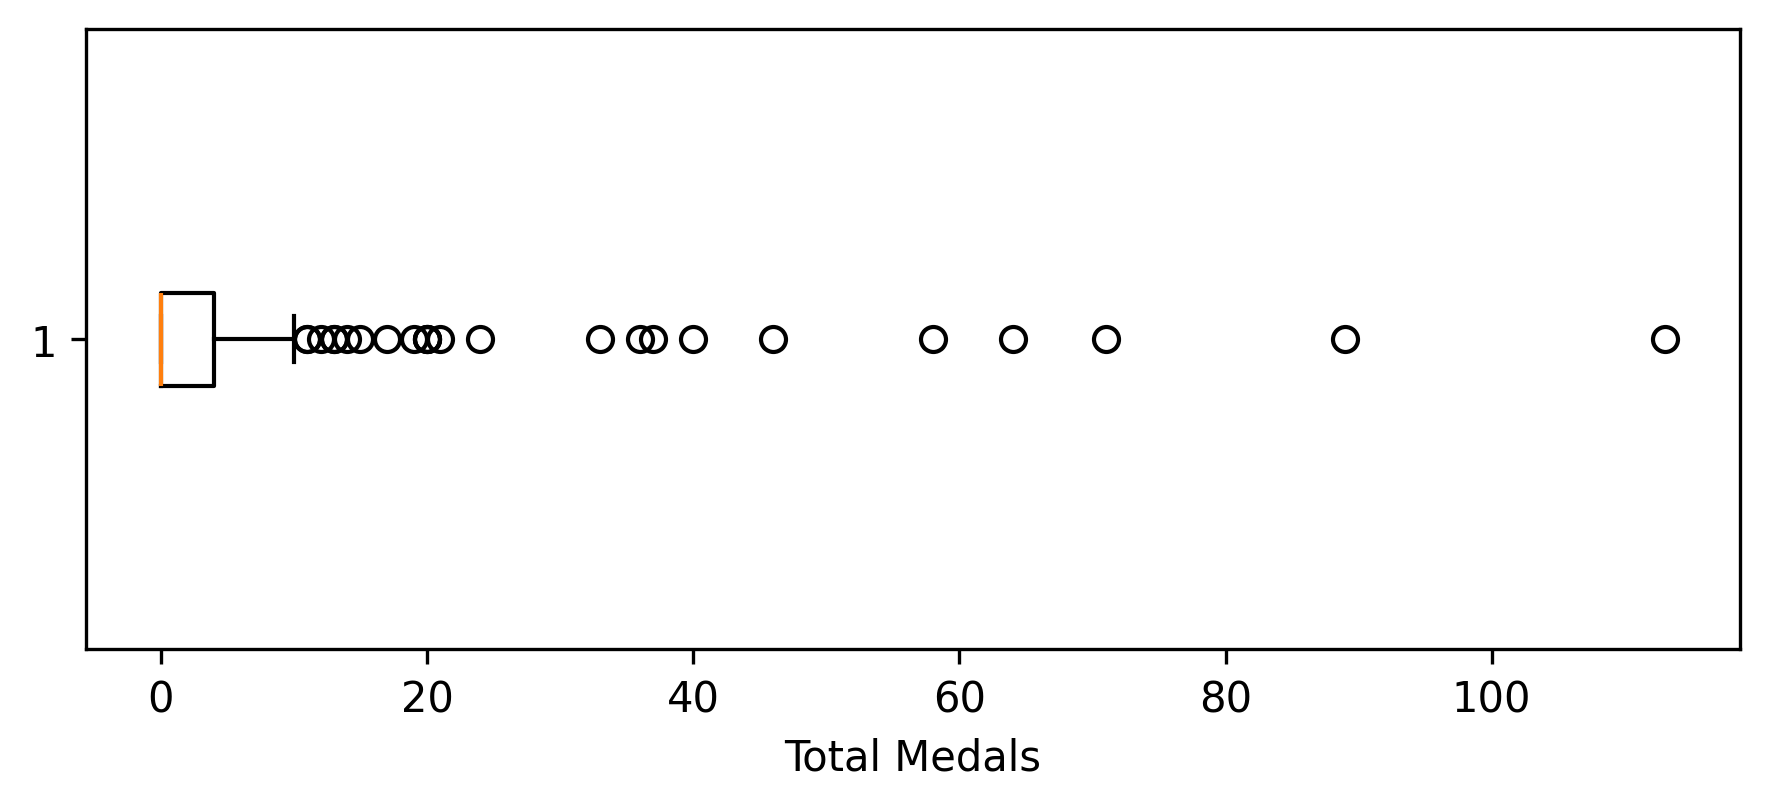
\includegraphics[width=0.8\textwidth]{totalmedals_box.png}
\caption{Box plot of Total medals at the Olympic Games Tokyo 2020}
\label{fig: Box plot of Total medals at the Olympic Games Tokyo 2020}
\end{figure}

To further contextualize these outliers, the top 20 NOCs ranked by total medals are presented in Figure~\ref{fig: Top 20 NOCs by Total Medals at the Olympic Games Tokyo 2020}. The United States leads with 113 medals, followed by China (88) and Russia (71), with the rest showing a gradual decline. The figure uses a blue gradient color scheme, in which darker shades correspond to higher medal counts, thereby visually emphasizing the dominance of the leading NOCs. The highest-ranked NOC is positioned at the top, and the clean layout—without unnecessary vertical or horizontal grid lines—ensures that the focus remains on the comparative differences in medal counts. This design enhances readability while maintaining the horizontal and vertical axes for accurate quantitative reference, making the visualization both aesthetically refined and analytically informative.

\begin{figure}[!ht]
\centering
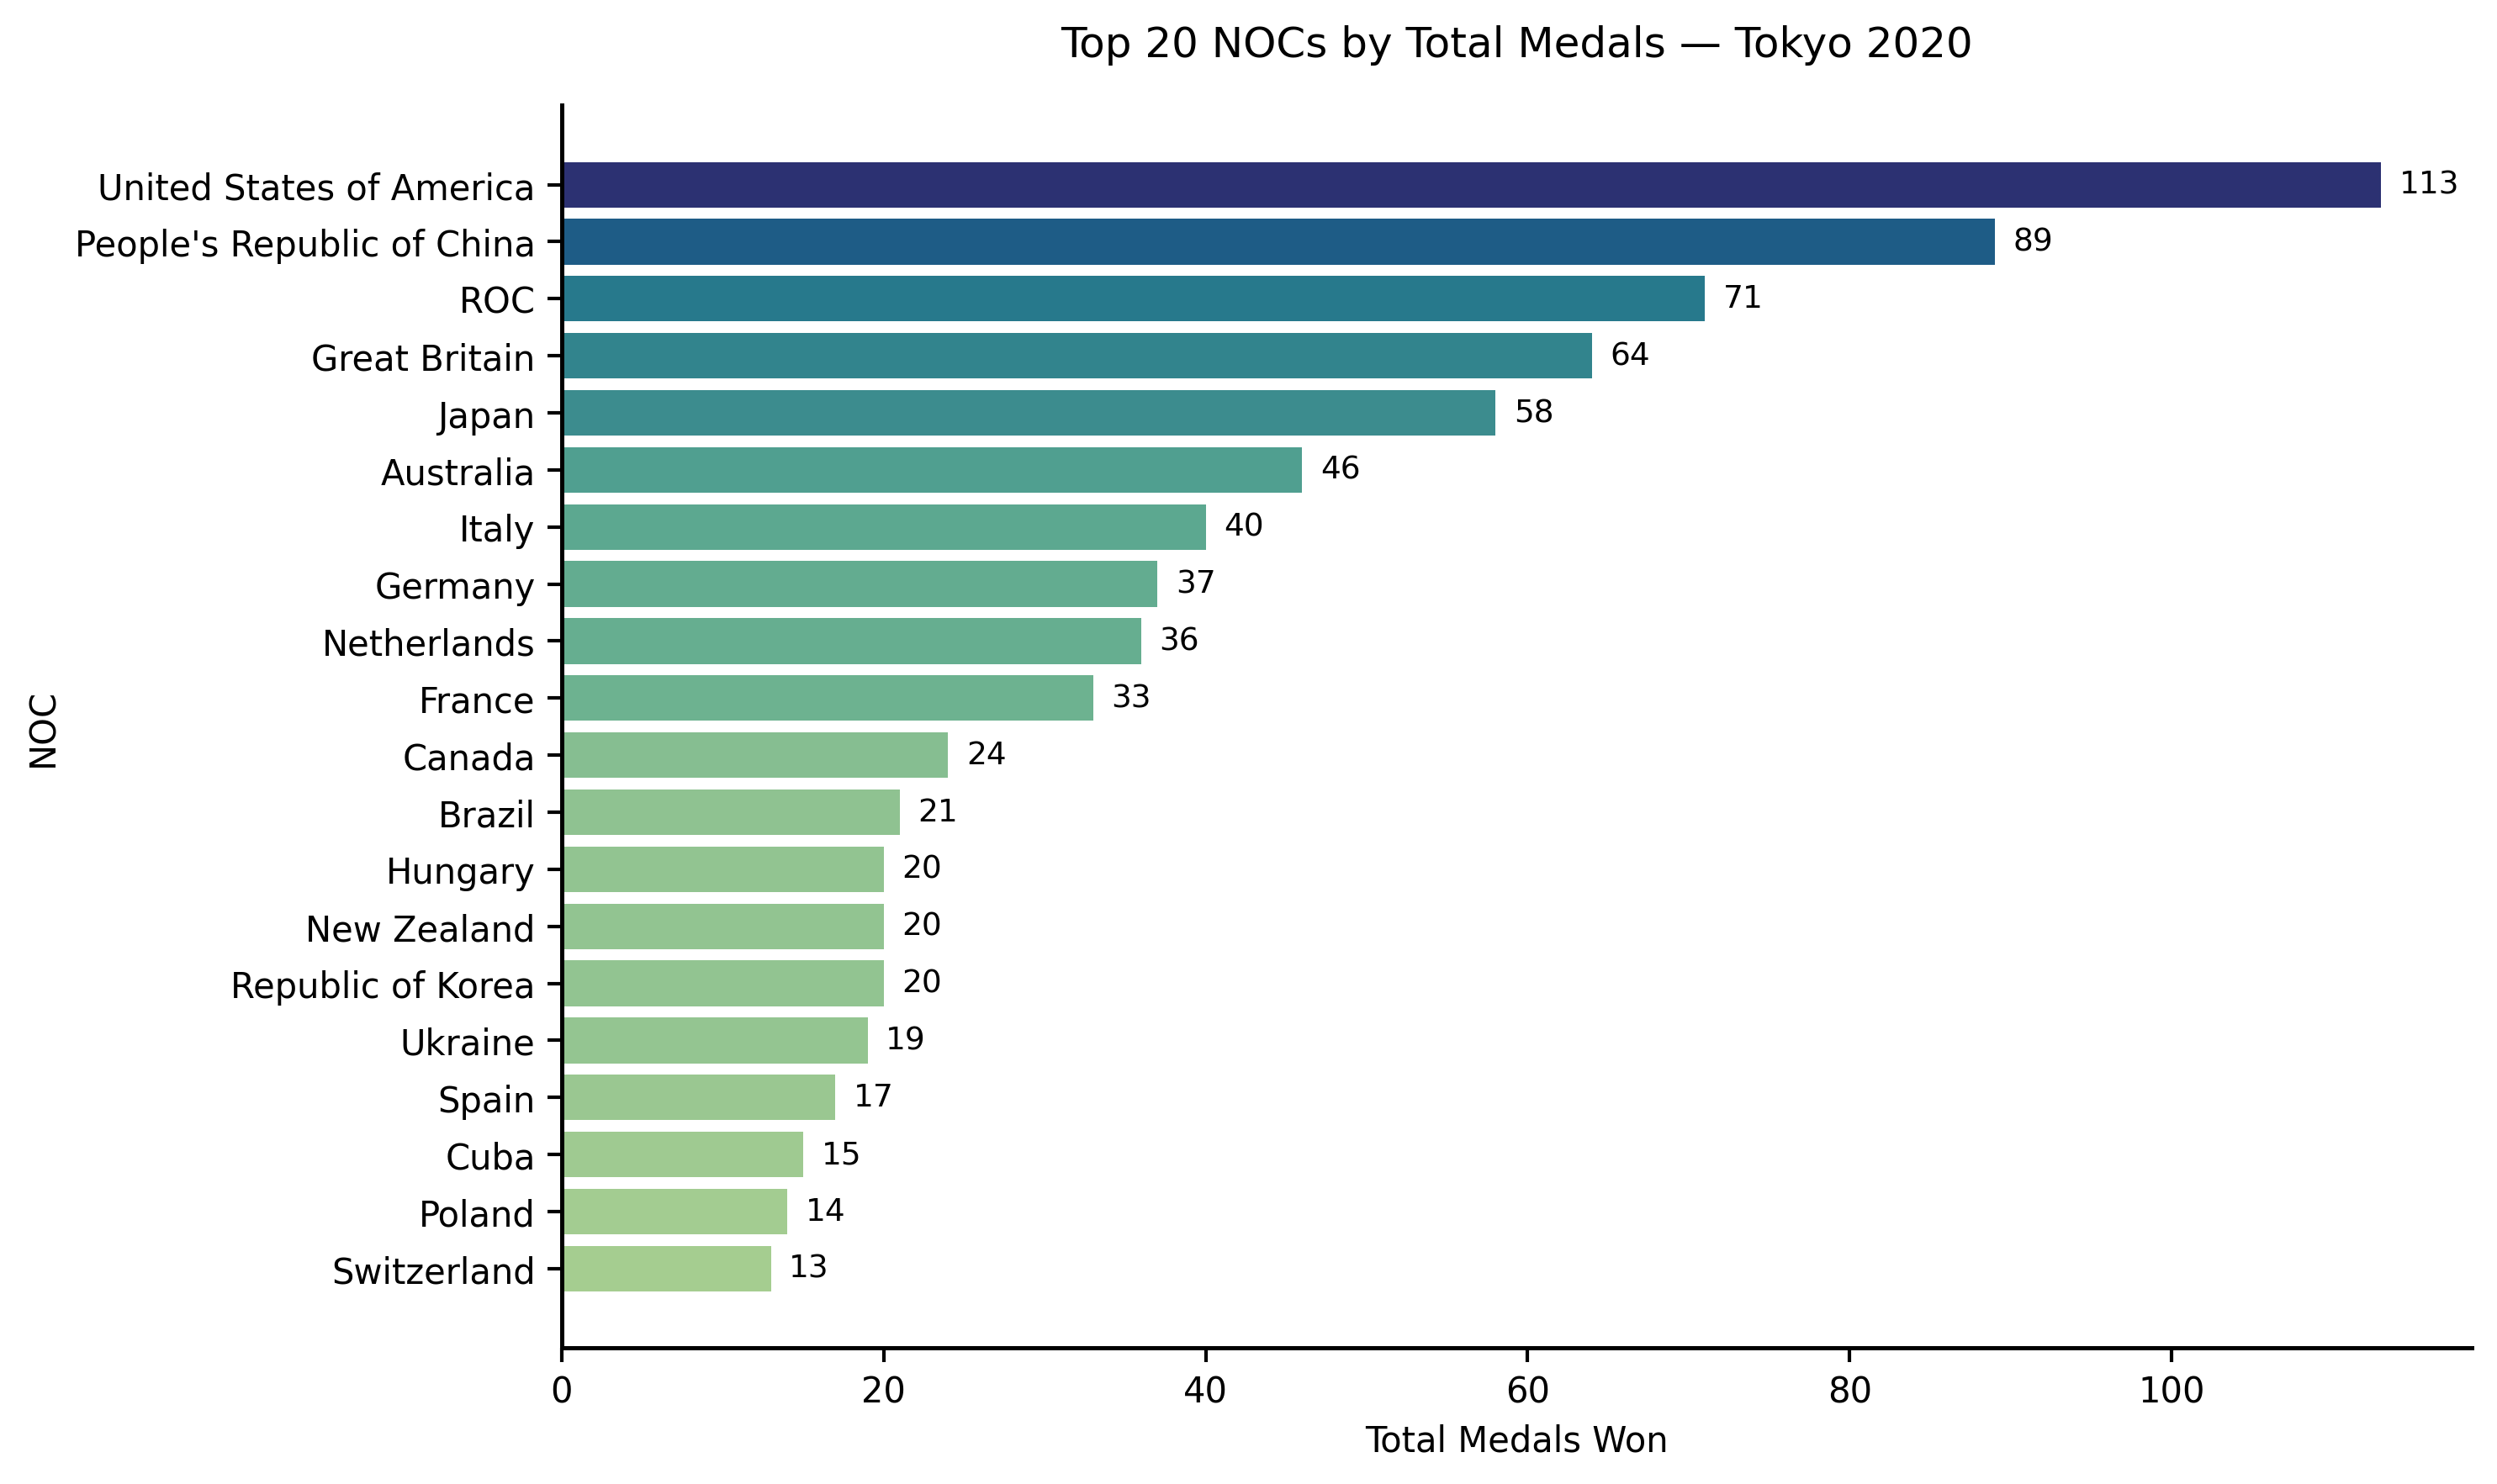
\includegraphics[width=0.8\textwidth]{top20_total_medals_axes_visible.png}
\caption{Top 20 NOCs by Total Medals at the Olympic Games Tokyo 2020}
\label{fig: Top 20 NOCs by Total Medals at the Olympic Games Tokyo 2020}
\end{figure}

In summary, the combined evidence from the zero-medal analysis, the box plot, and the top 20 ranking demonstrates a highly unequal distribution of Olympic medals, with a small group of NOCs capturing a disproportionate share. These findings underscore the importance of incorporating both zero inflation and skewness considerations into any statistical modeling of medal counts.

\subsubsection{Descriptive Statistics of Key Variables}

Table~\ref{tab:descriptive_statistics} presents the descriptive statistics for GDP, population, Human Development Index (HDI), number of athletes, and total medals across the participating National Olympic Committees (NOCs) in the Olympic Games Tokyo 2020, based on data from the year 2021. The results indicate substantial variability across these variables. GDP and population display extremely large standard deviations, reflecting pronounced disparities among countries, with certain nations possessing exceptionally high GDP despite relatively small populations (e.g., Qatar, Luxembourg). HDI values are comparatively concentrated, with a mean of 0.737, suggesting generally high human development levels among participating NOCs. The number of athletes exhibits a positively skewed distribution, where most NOCs sent relatively few competitors, while a small subset sent several hundred. Similarly, the total medal count is highly skewed, with a mean of 5.24 but a maximum of 113, underscoring the dominance of a limited number of medal-winning nations.

Notably, the total medal count variable contains a substantial proportion of zeros, as many NOCs did not secure any medals in the Olympic Games Tokyo 2020. This zero inflation, coupled with the evident right-skewness in the distribution of positive medal counts, suggests that conventional count models such as Poisson or negative binomial regression may not adequately capture the underlying data-generating process. Instead, these characteristics provide strong justification for considering zero-inflated regression models, which explicitly account for the excess zeros while modeling the distribution of non-zero counts.

Given the substantial magnitude and variability of GDP, population, and number of athletes, as evidenced by their large means and standard deviations in Table~\ref{tab:descriptive_statistics}, a log transformation was applied to these variables prior to further modeling. This transformation reduces skewness, mitigates the influence of extreme values, stabilizes variance, and facilitates the interpretability of model coefficients by placing these predictors on a comparable scale across NOCs.

\begin{table}[htbp]
\centering
\caption{Descriptive statistics of GDP, Population, HDI, Number of Athletes, and Total Medals}
\label{tab:descriptive_statistics}
\begin{tabular}{cccccc}
\toprule
\textbf{Variables} & \textbf{Mean} & \textbf{Median} & \textbf{Std Dev} & \textbf{Min} & \textbf{Max} \\
\midrule
GDP & 4.72715$\times 10^{11}$ & 3.23012$\times 10^{10}$ & 2.14255$\times 10^{12}$ & 3.7369$\times 10^{4}$ & 2.37$\times 10^{13}$ \\
Population & 3.90505$\times 10^{7}$ & 8.70455$\times 10^{6}$ & 1.45339$\times 10^{8}$ & 1.0194$\times 10^{4}$ & 1.41420$\times 10^{9}$ \\
HDI & 0.737 & 0.754 & 0.152 & 0.339 & 0.969 \\
Athletes & 55.947 & 10.5 & 104.581 & 2 & 621 \\
Totalmedals & 5.243 & 0 & 14.049 & 0 & 113 \\
\bottomrule
\end{tabular}
\end{table}

\begin{table}[htbp]
\centering
\caption{Descriptive statistics after log transformation for GDP, Population, and Athletes}
\label{tab:descriptive_statistics_log}
\begin{tabular}{cccccc}
\toprule
\textbf{Variables} & \textbf{Mean} & \textbf{Median} & \textbf{Std Dev} & \textbf{Min} & \textbf{Max} \\
\midrule
log(GDP)         & 24.255 &  24.197 &    2.565 & 10.529 &  30.796 \\
log(Population)  & 15.523 &  15.979 &    2.324 &  9.230 &  21.070 \\
log(Athletes)    &  2.786 &   2.350 &    1.549 &  0.693 &   6.431 \\
HDI              &  0.737 &   0.754 &    0.152 &  0.339 &   0.969 \\
Totalmedals      &  5.243 &   0.000 &   14.049 &  0.000 & 113.000 \\
\bottomrule
\end{tabular}
\end{table}

The log-transformed descriptive statistics in Table~\ref{tab:descriptive_statistics_log} show a marked reduction in the dispersion of GDP, population, and number of athletes compared with their original scales. The compression of extreme values is evident from the narrower standard deviations, particularly for GDP and population. This transformation not only improves numerical stability in subsequent regression modeling but also enhances the comparability of coefficients across predictors, thereby contributing to more robust and interpretable analytical results.

\subsubsection{Correlation Analysis of Predictors and Medal Counts}


Following the descriptive analysis, GDP, Population, and Athletes were log-transformed to mitigate skewness and enhance interpretability. Unless otherwise stated, all references to these variables henceforth use their transformed forms, namely $\log(\mathrm{GDP})$, $\log(\mathrm{Population})$, and $\log(\mathrm{Athletes})$, while HDI and total medals remain on their original scales.

The Pearson product-moment correlation coefficient measures the strength and direction of a \textbf{linear} relationship between two continuous variables\cite{pearson1896}. The Spearman rank correlation coefficient measures the strength and direction of a \textbf{monotonic} relationship based on ranks\cite{spearman1904}.

To assess associations among predictors and with the response (total medals), both Pearson’s product--moment correlation and Spearman’s rank correlation were computed on the set \{$\log(\mathrm{GDP})$, $\log(\mathrm{Population})$, HDI, $\log(\mathrm{Athletes})$, total medals\}. Figure~\ref{fig:corr_pearson_all} shows the Pearson matrix and Figure~\ref{fig:corr_spearman_all} shows the Spearman matrix.

\begin{figure}[htbp]
  \centering
  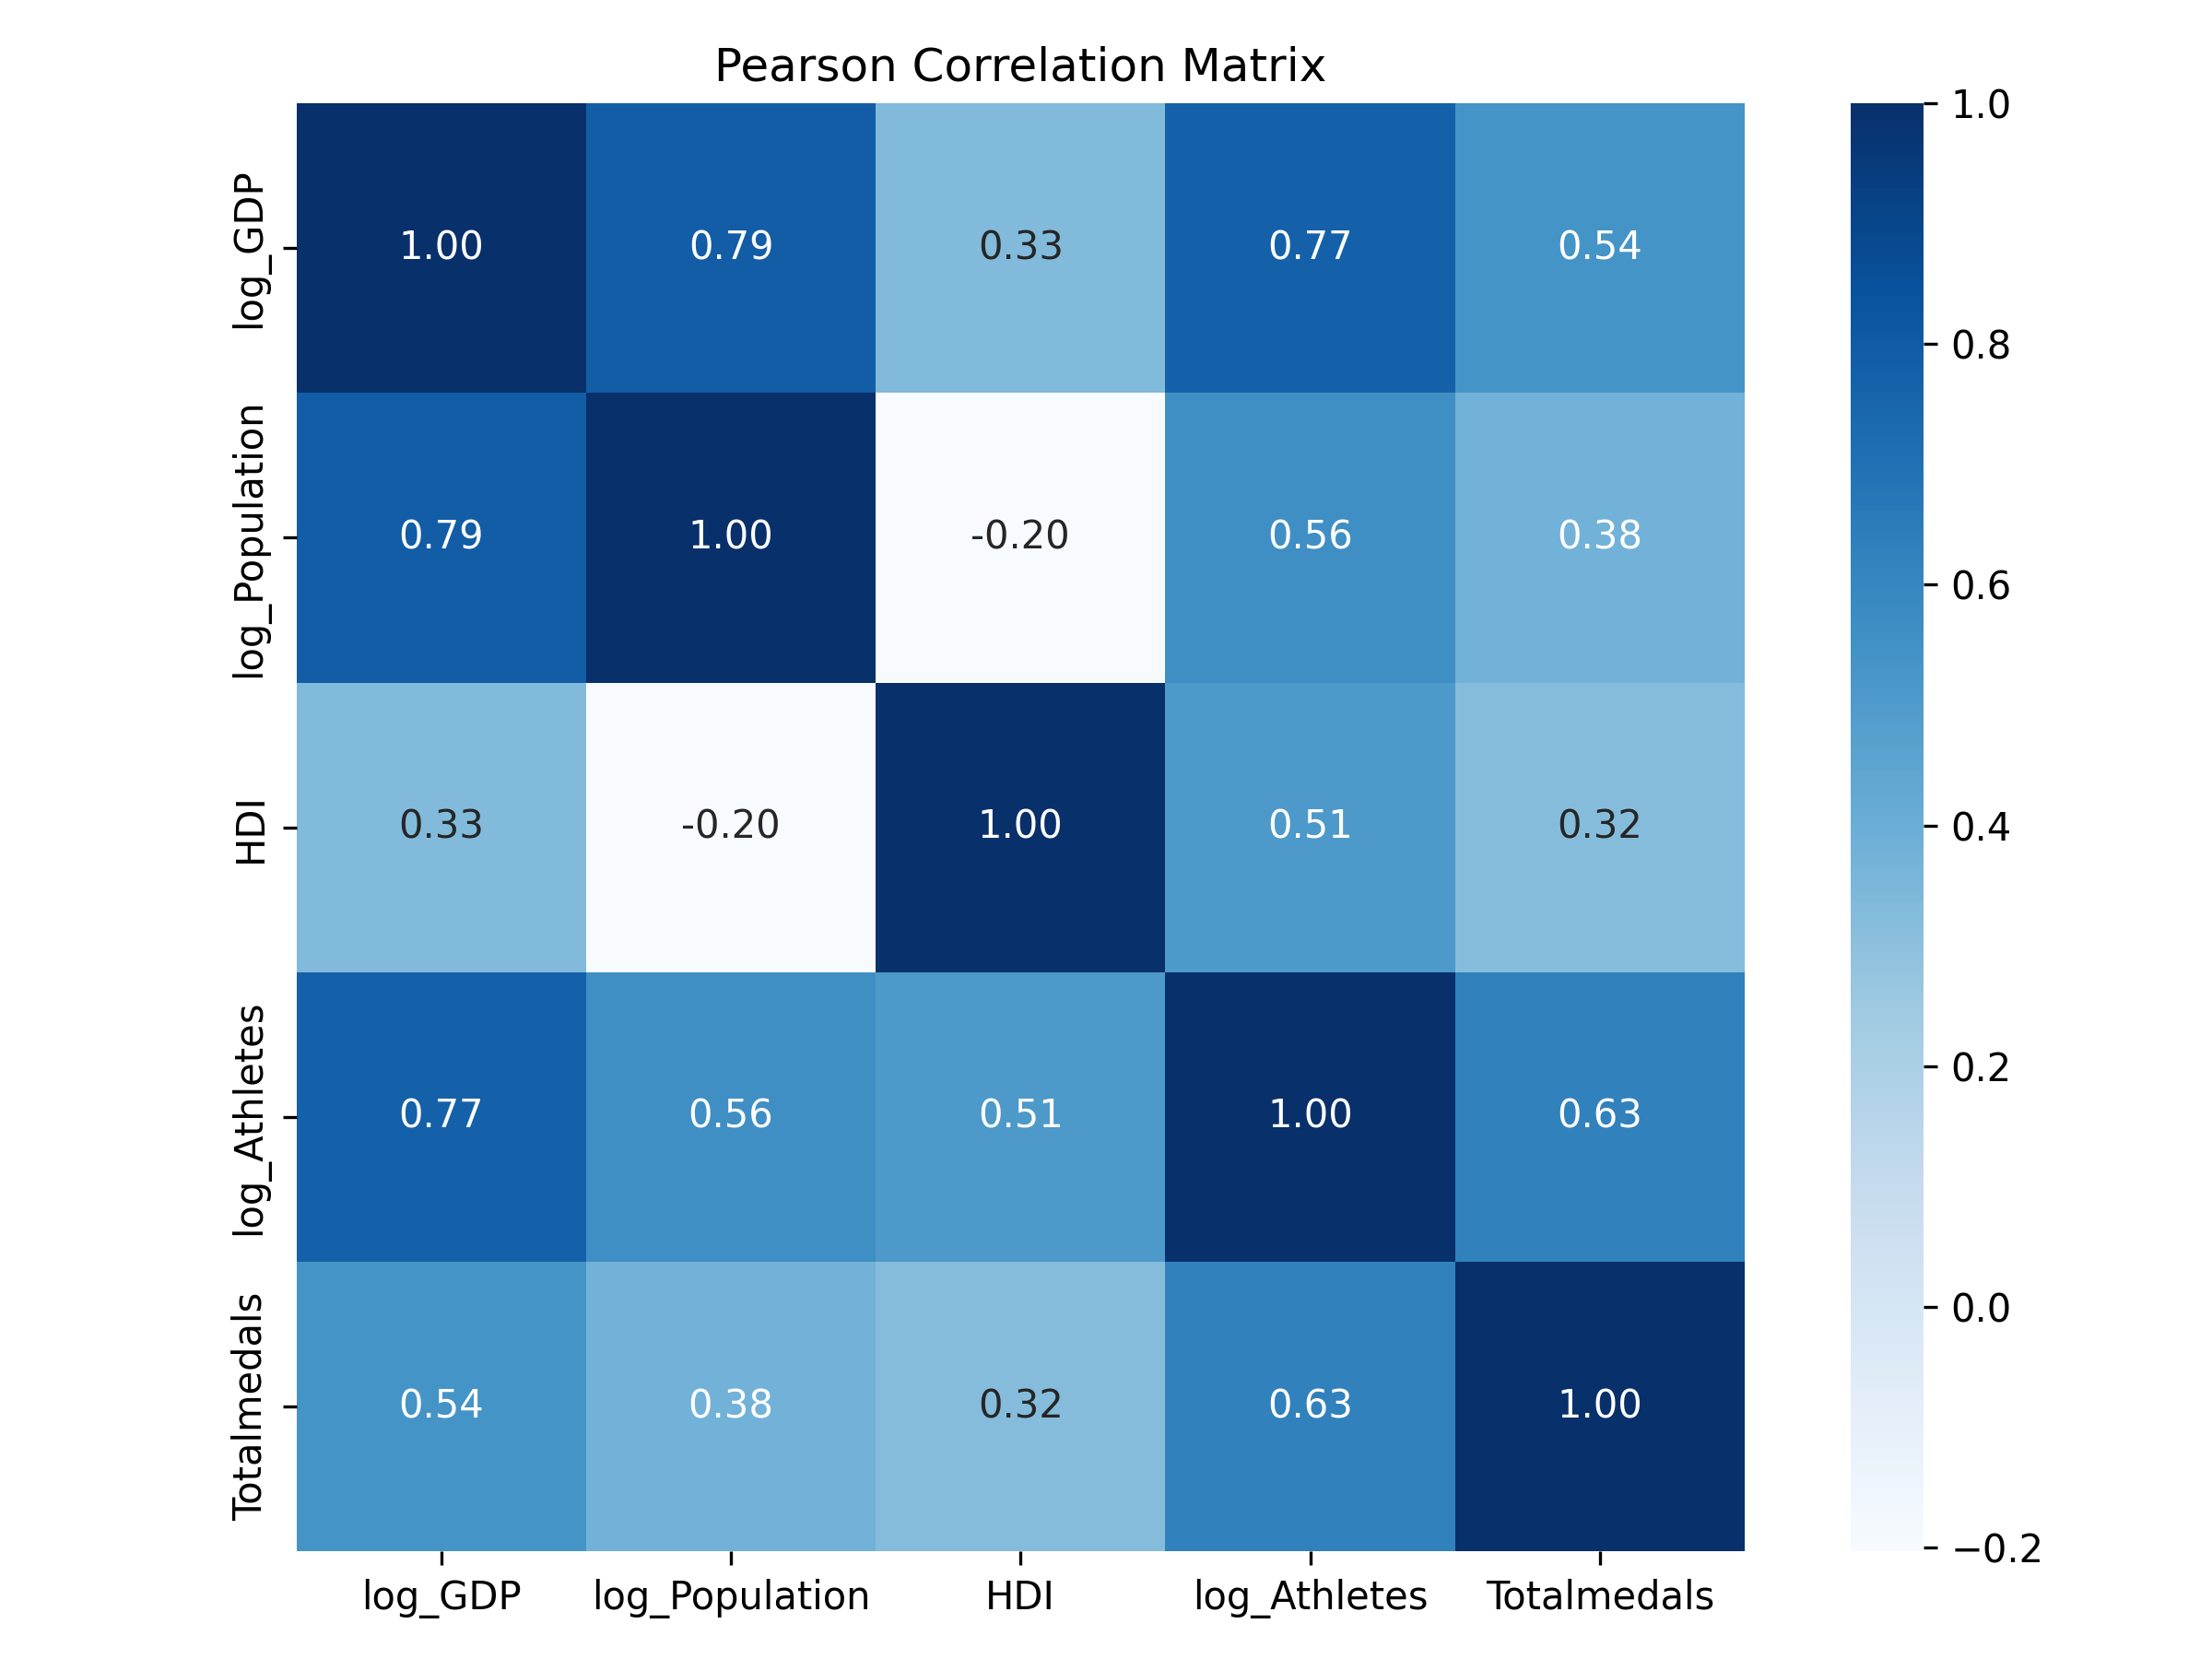
\includegraphics[width=0.78\textwidth]{pearson_correlation_matrix.png}
  \caption{Pearson correlation matrix for $\log(\mathrm{GDP})$, $\log(\mathrm{Population})$, HDI, $\log(\mathrm{Athletes})$, and total medals.}
  \label{fig:corr_pearson_all}
\end{figure}

\begin{figure}[htbp]
  \centering
  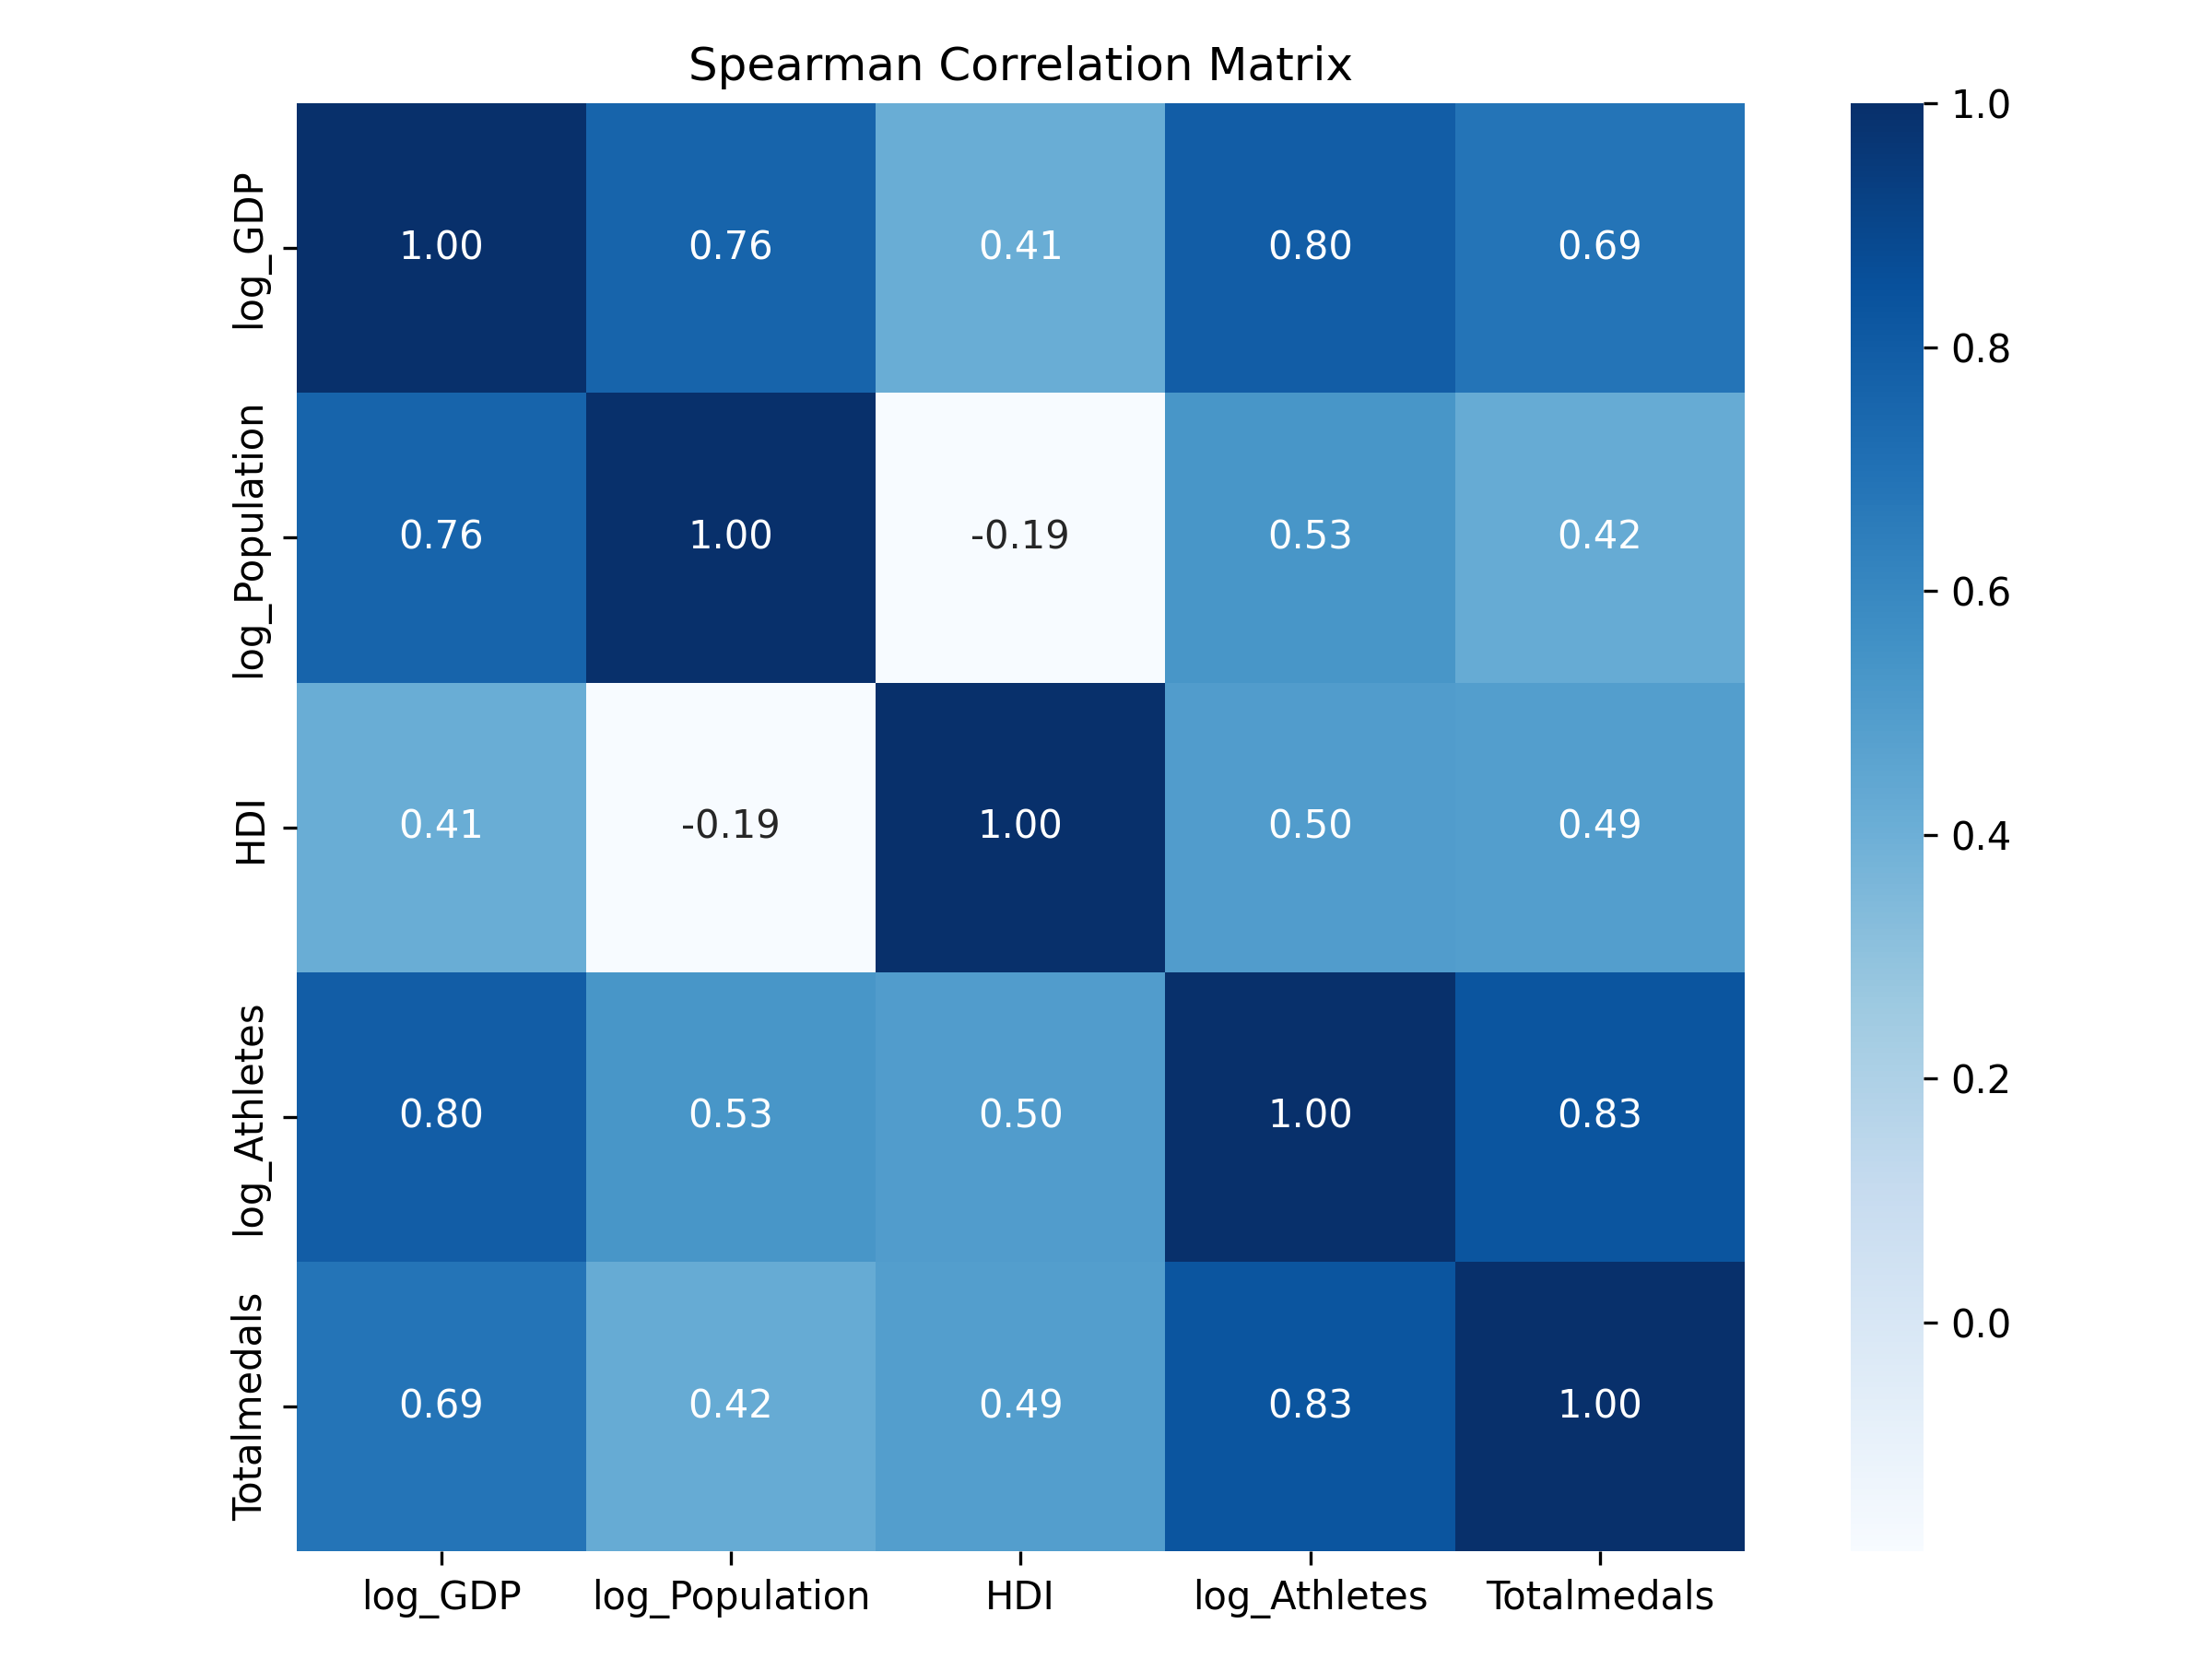
\includegraphics[width=0.78\textwidth]{spearman_correlation_matrix.png}
  \caption{Spearman correlation matrix for $\log(\mathrm{GDP})$, $\log(\mathrm{Population})$, HDI, $\log(\mathrm{Athletes})$, and total medals.}
  \label{fig:corr_spearman_all}
\end{figure}


Three robust patterns emerge from the correlation results. 
First, $\log(\mathrm{Athletes})$ shows the strongest association with total medals (Pearson $\approx 0.63$, Spearman $\approx 0.83$), indicating that delegation size is a primary driver of medal outcomes. 
Second, $\log(\mathrm{GDP})$ is also positively related to total medals (Pearson $\approx 0.54$, Spearman $\approx 0.69$), consistent with the idea that economic capacity supports elite sport systems. 
Third, HDI displays moderate positive associations with both $\log(\mathrm{Athletes})$ and total medals (Pearson $\approx 0.51/0.32$, Spearman $\approx 0.50/0.49$), suggesting that broader human development co-varies with participation and performance.

At the same time, notable dependencies exist among predictors: $\log(\mathrm{GDP})$ and $\log(\mathrm{Population})$ are strongly correlated (Pearson $\approx 0.79$, Spearman $\approx 0.76$), and $\log(\mathrm{Athletes})$ is substantially correlated with $\log(\mathrm{GDP})$ (Pearson $\approx 0.77$, Spearman $\approx 0.80$). These patterns motivate a formal multicollinearity check.

\subsubsection{Variance Inflation Factor Analysis of Predictors}

Variance Inflation Factor (VIF) is a diagnostic measure used to detect multicollinearity among independent variables in a regression model\cite{james2017isl}. 
It quantifies the extent to which the variance of an estimated regression coefficient is inflated due to linear relationships with other predictors. 

A VIF value of 1 indicates no correlation with other variables, whereas values exceeding commonly used thresholds of 5 suggest a high degree of multicollinearity\cite{sheather2009modern}, 
which can compromise the stability and interpretability of model coefficients. 
In this dissertation, VIF analysis is employed to ensure that the selected predictors exhibit acceptable levels of multicollinearity before inclusion in the main model.

Table~\ref{tab:vif_results} presents the Variance Inflation Factor (VIF) values for the log-transformed predictors considered in the subsequent modeling. 
All VIF values are below the commonly used threshold of 5, indicating that multicollinearity is not a severe concern in the dataset. 
Specifically, $\log(\mathrm{Athletes})$ exhibits the highest VIF of 3.89, followed by $\log(\mathrm{GDP})$ (3.21) and $\log(\mathrm{Population})$ (2.85), suggesting a moderate degree of correlation with other predictors. 
HDI shows the lowest VIF value (1.74), implying relatively low correlation with the remaining variables. 

The combined evidence from the correlation matrices and VIF diagnostics confirms that the selected predictors capture complementary aspects of economic, demographic, and developmental capacity, while maintaining acceptable levels of independence. 
Although certain variables, such as $\log(\mathrm{GDP})$ and $\log(\mathrm{Population})$, display relatively strong pairwise correlations, their VIF values remain below critical thresholds, indicating that collinearity is not severe enough to necessitate exclusion. 
Therefore, all four predictors --- $\log(\mathrm{GDP})$, $\log(\mathrm{Population})$, HDI, and $\log(\mathrm{Athletes})$ --- are retained for subsequent modeling, ensuring that the main model incorporates both scale-related and socio-developmental determinants of Olympic medal counts.


\begin{table}[htbp]
\centering
\caption{Variance Inflation Factor (VIF) for log-transformed predictors}
\label{tab:vif_results}
\begin{tabular}{cc}
\toprule
\textbf{Variable} & \textbf{VIF} \\
\midrule
log(GDP)         & 3.21 \\
log(Population)  & 2.85 \\
HDI              & 1.74 \\
log(Athletes)    & 3.89 \\
\bottomrule
\end{tabular}
\end{table}


\clearpage

% =============================================================================
% Modelling
% =============================================================================
\section{Modelling} 
\label{sec:modelling}

This chapter outlines the modelling approach, the rationale for model selection, the formal specification of the Zero-Inflated Negative Binomial (ZINB) model, and its software implementation.

\subsection{Model Selection}
\label{subsec:model_selection}

The distribution of medal counts among the 206 NOCs at the Tokyo 2020 Olympic Games exhibits clear count-data characteristics with both overdispersion and substantial structural zeros. The dependent variable, total medals per NOC, is a nonnegative integer with a highly skewed distribution. The mean is $\mu=5.24$, while the variance is $\sigma^2=196.41$, yielding a dispersion index of $\sigma^2/\mu=37.46$, which is far above the overdispersion threshold of 10 suggested by Cameron \citep{cameron2013}. This provides strong evidence of overdispersion. Moreover, 54.85\% of NOCs (113 out of 206) recorded zero medals, significantly exceeding the Poisson-expected zero rate $p_0 = e^{-\mu} \approx 0.0053$. A one-sided binomial test confirms this excess, with a p-value of $6.861 \times 10^{-198}$, thus indicating overwhelming structural zero inflation \citep{lambert1992, ridout2001}.

Classical count models face serious limitations in this setting. Poisson regression requires equality of mean and variance and thus fails under overdispersion \citep{cameron2013}. Negative Binomial (NB) regression accommodates overdispersion \citep{greene1994} but does not explicitly account for the zero-generating mechanism. Zero-Inflated Poisson (ZIP) models allow for structural zeros \citep{lambert1992}, yet still assume variance proportional to the mean, making them unsuitable for highly overdispersed data. To address both issues simultaneously, this dissertation adopts the \textbf{Zero-Inflated Negative Binomial (ZINB)} model \citep{greene1994}.

To provide a more intuitive explanation of the modelling rationale, Figure~\ref{fig:model_selection} presents a schematic framework illustrating the adoption of the ZINB model. 

\begin{figure}[H]
\centering
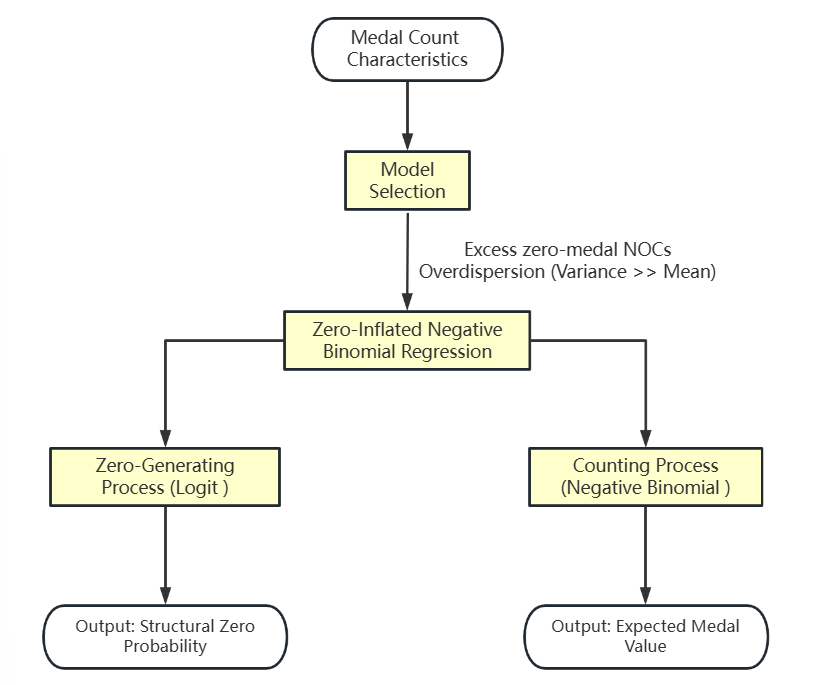
\includegraphics[width=0.8\textwidth]{flow chart.png}
\caption{Flowchart illustrating the rationale for selecting the Zero-Inflated Negative Binomial model, which jointly estimates the zero-generating and counting processes.}
\label{fig:model_selection}
\end{figure}


\subsection{Model Introduction}
\label{subsec:model_introduction}

The Zero-Inflated Negative Binomial (ZINB) model assumes that the observed medal count outcome $Y_i$ is generated from a mixture of two processes:  
\begin{enumerate}
    \item a \emph{zero-generating process}, which produces only structural zeros, i.e., countries or regions with no realistic chance of winning medals;  
    \item a \emph{count process}, which follows a Negative Binomial distribution and can generate both zeros and positive counts.  
\end{enumerate}

This dual specification simultaneously addresses two statistical challenges:  
(i) \textbf{overdispersion}, since the Negative Binomial component relaxes the Poisson equal-dispersion assumption via the parameter $\alpha$; and  
(ii) \textbf{zero inflation}, as the logit component models the probability of belonging to the structural-zero group.  

The probability mass function (PMF) is:  
\begin{equation}
P(Y_i = y_i) =
\begin{cases}
\pi_i + (1-\pi_i)\cdot f(0|\mu_i,r), & y_i = 0, \\
(1-\pi_i)\cdot f(y_i|\mu_i,r), & y_i > 0,
\end{cases}
\label{eq:zinb_pmf}
\end{equation}

where $f(y_i|\mu_i,r)$ denotes the Negative Binomial distribution:  
\[
f(y_i|\mu_i,r) = \frac{\Gamma(y_i + r)}{\Gamma(r)\,y_i!}
\left(\frac{r}{r+\mu_i}\right)^{r}
\left(\frac{\mu_i}{r+\mu_i}\right)^{y_i}.
\]

The model links are parameterized as follows:  
\begin{align}
\mu_i &= \exp(\mathbf{x}_i^\top \boldsymbol{\beta}), \label{eq:zinb_mu} \\
\pi_i &= \frac{\exp(\mathbf{z}_i^\top \boldsymbol{\gamma})}{1 + \exp(\mathbf{z}_i^\top \boldsymbol{\gamma})}, \label{eq:zinb_pi} \\
r &= \frac{1}{\alpha}, \label{eq:zinb_r}
\end{align}

where $\mu_i$ is the conditional mean under the count process, $\pi_i$ is the probability of belonging to the structural-zero group, and $r$ is the shape parameter of the Negative Binomial distribution, inversely related to the overdispersion parameter $\alpha$.

\subsubsection{Variable Definitions}

In this dissertation, the variables are defined as follows:  
\begin{itemize}
    \item $Y_i$: Total number of medals won by NOC $i$ at the Tokyo 2020 Olympic Games.  
    \item $\mathbf{x}_i$: Predictors for the count process, including:  
    \begin{itemize}
        \item $\log(\mathrm{GDP}_i)$: Natural logarithm of Gross Domestic Product.  
        \item $\log(\mathrm{Population}_i)$: Natural logarithm of population size.  
        \item $\mathrm{HDI}_i$: Human Development Index (0--1 scale).  
        \item $\log(\mathrm{Athletes}_i)$: Natural logarithm of the number of athletes.  
    \end{itemize}
    \item $\boldsymbol{\beta}$: Regression coefficients for the count process, capturing the effect of predictors on expected medal counts.  
    \item $\mathbf{z}_i$: Predictors for the zero-generating process (set identical to $\mathbf{x}_i$ in this study).  
    \item $\boldsymbol{\gamma}$: Regression coefficients for the zero-generating process, reflecting the influence of predictors on the log-odds of being a structural zero.  
    \item $\mu_i$: Conditional mean of medal counts given the count process.  
    \item $\pi_i$: Probability that NOC $i$ belongs to the structural-zero group.  
    \item $\alpha$: Overdispersion parameter; larger values imply greater variance inflation relative to Poisson.  
\end{itemize}

Note: In the count equation, coefficients $\beta$ can be interpreted as elasticities or semi-elasticities. For instance, if the GDP coefficient equals 0.3, then a 10\% increase in GDP corresponds to an approximate 3\% increase in expected medal counts. In the zero-generating equation, the sign of $\gamma$ indicates whether a predictor increases or decreases the likelihood of observing zero medals.  

\subsubsection{Model Estimation}

The ZINB model jointly estimates $\boldsymbol{\beta}$, $\boldsymbol{\gamma}$, and $\alpha$ via maximum likelihood estimation (MLE) \citep{seabold2010}. The likelihood function integrates contributions from both the zero-generating and count processes, and maximization requires iterative numerical optimization (e.g., L-BFGS), since no closed-form solution exists.  

Model evaluation relies on two widely used information criteria. The first is the Akaike Information Criterion (AIC) \citep{akaike1974}, which balances model fit against complexity:  
\begin{equation}
\mathrm{AIC} = -2\ell_{\max} + 2k,
\label{eq:aic}
\end{equation}
where $\ell_{\max}$ is the maximized log-likelihood and $k$ is the number of estimated parameters. AIC tends to favor models with good predictive accuracy, particularly in finite samples.  

As a complementary measure, the Bayesian Information Criterion (BIC) \citep{schwarz1978} is also employed:  
\begin{equation}
\mathrm{BIC} = -2\ell_{\max} + k \cdot \ln(n),
\label{eq:bic}
\end{equation}
where $n$ denotes the sample size. Compared to AIC, BIC applies a stricter penalty on model complexity, especially as $n$ increases. Rooted in Bayesian principles, BIC provides consistent model selection in large samples, and thus tends to prefer more parsimonious specifications, reducing the risk of overfitting.  

By considering both AIC and BIC, this study achieves a balanced assessment between model fit and parsimony. In the empirical analysis, both criteria will be reported to provide comprehensive evidence for model adequacy.  


% =========================
% Section 3.3 (aligned with your structure)
% =========================
\subsection{Software Implementation}
\label{subsec:software}

\subsubsection{Software Environment and Reproducibility}
All computations were conducted on \textbf{Windows 11 (x64)} using \textbf{Python 3.12.7}. Model estimation relied primarily on \texttt{statsmodels 0.14.4}, with \texttt{numpy 2.0.2} and \texttt{pandas 2.2.3} for numerical operations, \texttt{scipy 1.14.1} for optimization and statistical testing, and \texttt{openpyxl 3.1.5} for file export. To ensure reproducibility, the random seed was fixed at 123. The estimator employed was \texttt{ZeroInflatedNegativeBinomialP} (NB2 parameterization) from \texttt{statsmodels}. The raw dataset (\texttt{dataset1.xlsx}) and prediction outputs (\texttt{zinb\_predictions.csv}) are provided in the Appendix for replication.

\subsubsection{Model Implementation and Estimation}
The count process was parameterized with a log link:
\begin{equation}
\log(\mu_i) = a + b \log(\mathrm{GDP}_i) + c \log(\mathrm{Population}_i) + d \mathrm{HDI}_i + e \log(\mathrm{Athletes}_i).
\label{eq:count_link}
\end{equation}

The zero-generating process was specified with a logit link:
\begin{equation}
\pi_i = \gamma_0 + \gamma_1 \log(\mathrm{GDP}_i) + \gamma_2 \log(\mathrm{Population}_i) + \gamma_3 \mathrm{HDI}_i + \gamma_4 \log(\mathrm{Athletes}_i).
\label{eq:logit_link}
\end{equation}

Parameters were estimated via maximum likelihood, with the L-BFGS algorithm (maximum 600 iterations) as the primary optimizer. If convergence was not achieved, BFGS was used as an alternative. The overall computational procedure, from data input and parameterization to estimation and diagnostics, is summarized in Algorithm~\ref{alg:zinb}. This schematic not only illustrates the rationale for adopting the ZINB model but also clarifies the logical structure of its software implementation.

\begin{algorithm}[t]
\caption{ZINB Fitting and Prediction Pipeline}
\label{alg:zinb}
\begin{algorithmic}[1]
\Require Excel file $f$, required columns $\{\texttt{Totalmedals},\texttt{GDP},\texttt{Population},\texttt{HDI},\texttt{Athletes}\}$
\Ensure Table with $\pi$, $\mu$, $\mathbb{E}[Y]$, standardized residual $r$ for each NOC
\Function{FitZINBAndPredict}{$f$}
  \State $D \gets \Call{ReadExcel}{f}$
  \ForAll{$c$ in required columns} \Comment{safe numeric casting}
     \State $D[c] \gets \Call{ToNumericClean}{D[c]}$
  \EndFor
  \State $D \gets \Call{DropNA}{D, \text{required columns}}$
  \State $D \gets \{\,\text{rows}: \texttt{GDP}>0,\ \texttt{Population}>0,\ \texttt{Athletes}>0\,\}$
  \State $g \gets \log(\texttt{GDP}),\ p \gets \log(\texttt{Population}),\ a \gets \log(\texttt{Athletes}),\ h \gets \texttt{HDI}$
  \State $y \gets \texttt{Totalmedals}$
  \State $X \gets [\mathbf{1}, g, p, h, a]$ \Comment{count part (log link)}
  \State $Z \gets [\mathbf{1}, g, p, h, a]$ \Comment{inflation part (logit link)}
  \State $(\hat\theta,\hat\alpha) \gets \Call{ZINB\_MLE}{y,X,Z,\text{inflation}=\text{logit}}$ \Comment{try L-BFGS; fallback BFGS}
  \State $(a_0,b,c,d,e) \gets \Call{ExtractCountCoeffs}{\hat\theta}$
  \State $\mu \gets \exp(a_0 + b g + c p + d h + e a)$
  \State $\pi \gets \Call{Predict}{\hat\theta; X,Z,\text{which}=\text{prob-zero}}$
  \State $\mathbb{E}[Y] \gets (1-\pi)\cdot \mu$
  \State $\mathrm{Var}_{NB} \gets \mu + \hat\alpha\,\mu^2$
  \State $\mathrm{Var}(Y) \gets (1-\pi)\cdot \mathrm{Var}_{NB} + \pi(1-\pi)\mu^2$
  \State $r \gets (y-\mathbb{E}[Y])\,/\,\sqrt{\mathrm{Var}(Y)+\varepsilon}$ \Comment{$\varepsilon$ avoids division by zero}
  \State \Return $\{\texttt{Code},\texttt{Team},y,g,p,h,a,\pi,\mu,\mathbb{E}[Y],r\}$
\EndFunction
\end{algorithmic}
\end{algorithm}


\subsubsection{Interpretation and Diagnostics}
From the fitted model, the expected value and variance of medal counts are given by:
\begin{align}
E[Y_i] &= (1 - \pi_i)\mu_i, \label{eq:expected_value}\\
Var(Y_i) &= (1 - \pi_i)(\mu_i + \alpha \mu_i^2) + \pi_i (1 - \pi_i)\mu_i^2. \label{eq:variance}
\end{align}

Finally, standardized residuals were computed as:
\begin{equation}
r_i = \frac{Y_i - (1 - \pi_i)\mu_i}{\sqrt{(1 - \pi_i)(\mu_i + \alpha \mu_i^2) + \pi_i(1 - \pi_i)\mu_i^2}}.
\label{eq:residual}
\end{equation}

In the count equation, coefficients of GDP, Population, and Athletes can be interpreted as elasticities. For instance, if $\beta_{\text{GDP}} = 0.3$, then a 10\% increase in GDP corresponds to an approximate 3\% increase in expected medal counts. The HDI coefficient is a semi-elasticity: for example, a 0.1 increase in HDI (e.g., from 0.7 to 0.8) changes expected medal counts by approximately $\exp(0.1 \cdot \beta_{HDI}) - 1$.  

In the zero-generating equation, coefficients capture the likelihood of observing zero medals. A negative coefficient reduces the probability of being a structural zero, implying a higher likelihood of winning at least one medal.  

All outputs, including predictions, residuals, and diagnostic indicators, were exported as CSV files for further analysis and visualization.


\section{Results and Analysis}
\subsection{ZINB Model Result Analysis and Fitting Statistics}

Table~\ref{tab:zinb_coef} presents the estimates for the Zero-Inflated Negative Binomial (ZINB) model, with two main components: the count component (log link) and the inflation component (logit link). The count component models the expected total number of medals, while the inflation component models the probability of a structural zero.

\begin{table}[H]
\centering
\caption{Zero-Inflated Negative Binomial (ZINB) estimates: count vs.\ inflation components}
\label{tab:zinb_coef}
\begin{tabular}{lrrrrrr}
\toprule
\multicolumn{7}{c}{\textbf{Panel A: Count component (log link)}}\\
\midrule
Variable & Coef. & Std. Err. & $z$ & $p$-value & \multicolumn{2}{c}{95\% CI / IRR} \\
\cmidrule(lr){6-7}
 &  &  &  &  & [2.5\%, 97.5\%] & IRR = $\exp(\beta)$ \\
\midrule
Constant             &  -3.07 & 1.42 & -2.16 & 0.03 & [-5.87,\,-0.28] & 0.05 \\
$\log(\mathrm{GDP})$ &  -0.18 & 0.17 & -1.08 & 0.28 & [-0.52,\,0.15]  & 0.83 \\
$\log(\mathrm{Pop})$ &   0.20 & 0.18 &  1.13 & 0.26 & [-0.15,\,0.56]  & 1.23 \\
$\mathrm{HDI}$       &   1.93 & 1.97 &  0.98 & 0.33 & [-1.92,\,5.78]  & 6.88 \\
$\log(\mathrm{Ath})$ &   1.10 & 0.13 &  8.34 & 0.00 & [0.85,\,1.36]   & 3.02 \\
\midrule
NB dispersion $\alpha$ & 0.21 & 0.06 & 3.72 & 0.00 & [0.10,\,0.33] & \\
\addlinespace[2pt]
\multicolumn{7}{c}{\textbf{Panel B: Inflation component (logit link)}}\\
\midrule
Variable & Coef. & Std. Err. & $z$ & $p$-value & \multicolumn{2}{c}{95\% CI / OR} \\
\cmidrule(lr){6-7}
 &  &  &  &  & [2.5\%, 97.5\%] & OR $=\exp(\gamma)$ \\
\midrule
inflate\_const           & 10.67 & 8.35 &  1.28 & 0.20 & [-5.68,\,27.03] & $4.30\times 10^{4}$ \\
inflate\_log\_GDP        & -1.66 & 0.78 & -2.13 & 0.03 & [-3.18,\,-0.13] & 0.19 \\
inflate\_log\_Pop        &  1.61 & 0.79 &  2.03 & 0.04 & [0.06,\,3.15]   & 4.98 \\
inflate\_HDI             &  9.77 & 8.06 &  1.21 & 0.23 & [-6.02,\,25.56] & $1.75\times 10^{4}$ \\
inflate\_log\_Athletes   & -1.40 & 0.59 & -2.37 & 0.02 & [-2.57,\,-0.24] & 0.25 \\
\bottomrule
\end{tabular}
\end{table}

\subsubsection{Analysis of the Counting Part of the ZINB Model}

In the count equation, the coefficient on $\log(\mathrm{Athletes})$ is positive and statistically significant (about 1.10), indicating that---conditional on GDP, Population, and HDI---the scale of participation is the \textbf{dominant driver} of the expected medal count. By contrast, the coefficients on $\log(\mathrm{GDP})$ and $\log(\mathrm{Population})$ are small and not significant (slightly negative and slightly positive, respectively), and the HDI coefficient is positive but imprecise. This pattern suggests that once participation is controlled for, macro indicators add little incremental explanatory power. The estimated NB dispersion parameter $\alpha>0$ is significant, confirming \textbf{overdispersion} and justifying the NB2 variance instead of Poisson.


\subsubsection{Analysis of the Expansion Part of the ZINB model}

In the inflation equation (log-odds of a structural zero), $\log(\mathrm{GDP})$ and $\log(\mathrm{Athletes})$ enter with significant negative signs (odds ratios $<1$), implying that larger economic size and sending more athletes reduce the risk of zero medals. In contrast, $\log(\mathrm{Population})$ is significantly positive (odds ratio $>1$), indicating that, conditional on GDP, HDI, and participation, sheer population size does \emph{not} proxy for participation and may be associated with a higher zero risk. The HDI effect in the inflation part is not significant, consistent with development operating mainly through participation/investment channels. Overall, participation drives the post-entry scale of medals, GDP improves entry, Population adds little once athletes are accounted for, and HDI’s positive effect lacks robust significance.




\subsubsection{Analysis of ZINB Model Fit Statistics}
\label{subsubsec:zinb-model-fit}

In this section, the statistics involved include pseudo-\( R^2 \), likelihood ratio test p-value (LLR p-value), Akaike Information Criterion (AIC), and the dispersion parameter \(\alpha\) of the negative binomial distribution. These statistics are used to evaluate the goodness of fit and validity of the Zero-Inflated Negative Binomial (ZINB) model.

Pseudo-\( R^2 \) is a measure of model fit, especially useful in generalized linear models (GLM). It is calculated by comparing the log-likelihood of the model to the log-likelihood of a baseline model (typically the intercept-only model). The value of pseudo-\( R^2 \) typically ranges between 0 and 1, with higher values indicating a better fit to the model \cite{McFadden1974}.

The likelihood ratio test is used to compare the log-likelihoods of the complex and simpler models to test the statistical significance of the model. The lower the p-value, the higher the statistical significance of the model. Generally, a p-value less than 0.05 or 0.01 indicates that the results of the model are statistically significant \cite{Wilks1938}.

The dispersion parameter \(\alpha\) of the negative binomial distribution measures the degree of overdispersion in the data. In the negative binomial regression model, the size of \(\alpha\) reveals the difference between the variability in the data and what a Poisson distribution would expect. When \(\alpha\) is close to 0, the negative binomial distribution approaches the Poisson distribution, indicating that the data do not exhibit overdispersion; when \(\alpha\) is larger, it indicates greater overdispersion \cite{Nelder1972}.


Table~\ref{tab:zinb_fit} summarizes the model fit statistics for the ZINB model in this dissertation. The pseudo-$R^2$ is 0.34, indicating a relatively modest fit, although the extremely small LLR p-value (3.59 × 10$^{-63}$) suggests that the model is highly statistically significant. This indicates that despite a limited fit, the model provides a strong distinction between structural zeros and medal counts.

\begin{table}[H]
\centering
\caption{ZINB model fit statistics}
\label{tab:zinb_fit}
\begin{tabular}{l r}
\toprule
No.\ of observations & 206 \\
Log-likelihood & -294.12 \\
AIC & 610.24 \\
Pseudo-$R^2$ & 0.34 \\
LLR $p$-value & $3.59\times 10^{-63}$ \\
NB dispersion $\alpha$ & 0.21 \\
Covariance type & nonrobust \\
\bottomrule
\end{tabular}
\end{table}

Furthermore, the AIC value of 610.24 suggests that this model strikes a good balance between fit and complexity, performing well among the alternative model specifications. The negative binomial dispersion parameter $\alpha$ is estimated at 0.21, confirming the presence of overdispersion, which means that the variance in the data exceeds what would be predicted by a Poisson distribution. Finally, the model uses the "nonrobust" covariance type, which may imply that standard error estimates could be biased, and caution should be exercised in applying the model's results directly in some contexts.


\subsection{Residual Distribution}
\subsubsection{Distributional Features of Standardized Residuals}

Figure~\ref{fig:resid_hist} depicts the histogram and kernel density of the standardized
residuals, $r_i=\{y_i-\widehat{\mathbb{E}}[Y_i]\}/\sqrt{\widehat{\mathrm{Var}}(Y_i)}$.
The distribution is centered at zero with a pronounced peak, and the majority of
observations lie within the conventional band $|r_i|\leq2$, indicating acceptable fit
for most NOCs. At the same time, the density is clearly \emph{right-skewed} with a
\emph{heavy right tail}: several observations exceed $r_i>3$, implying that for a small
set of countries the realized medal counts are substantially higher than the model-based
expectations (i.e., underprediction for top performers). Relative to the normal reference
density calibrated by the sample mean and variance, the kernel density is sharper at the
center and thicker in the right tail, signaling a deviation from symmetry and normality.
This pattern is consistent with the highly concentrated nature of Olympic medals and the
heterogeneity of headlined teams.

\begin{figure}[H]
  \centering
  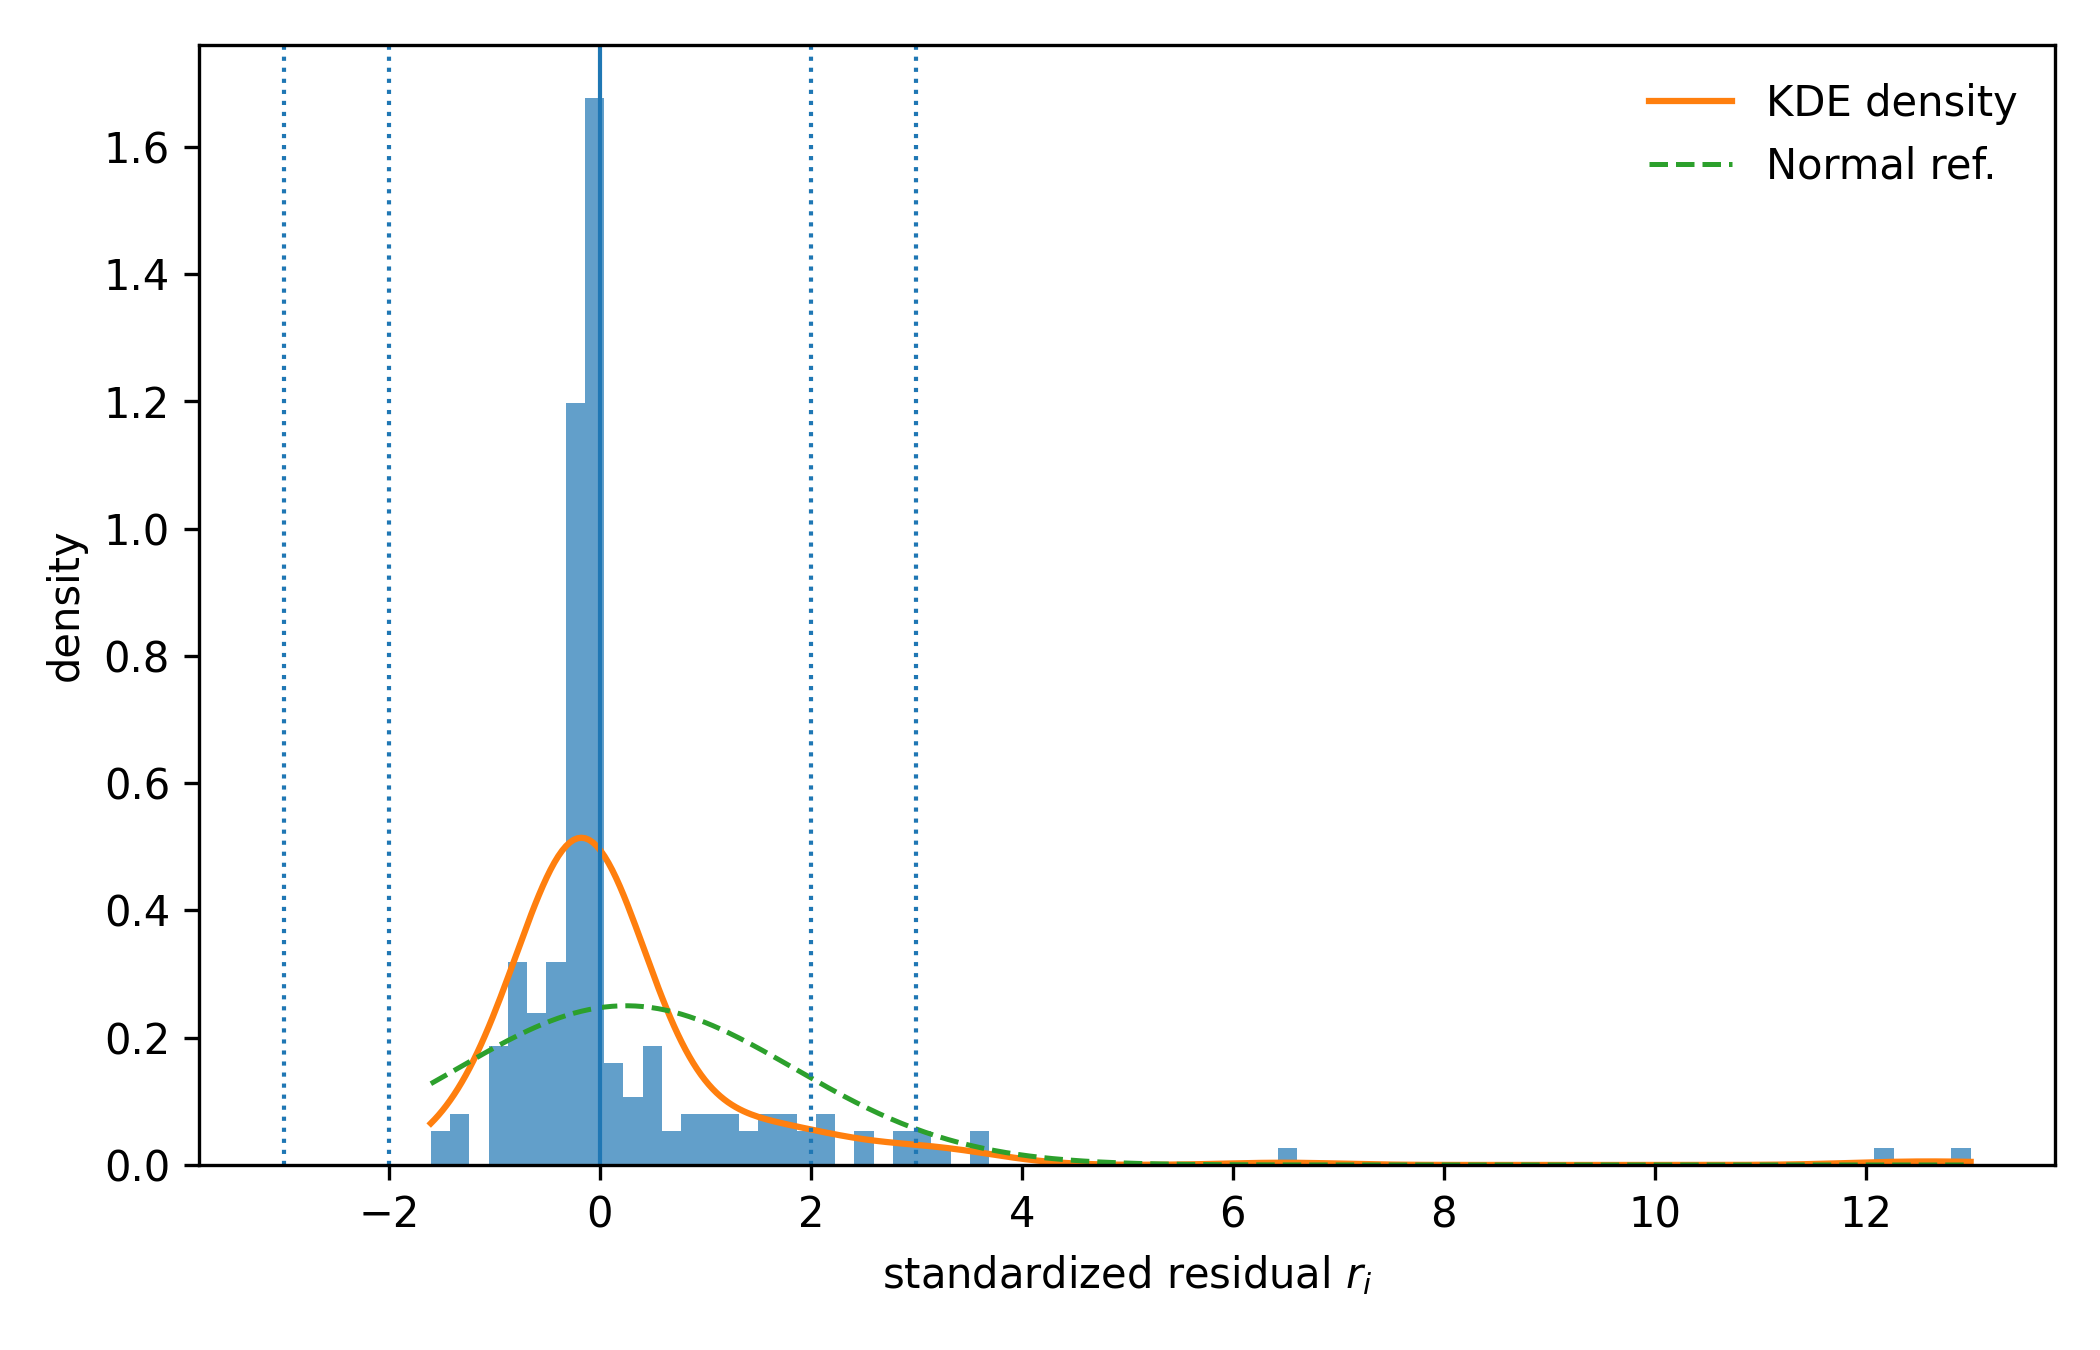
\includegraphics[width=0.92\linewidth]{fig_resid_hist.png}
  \caption{Standardized residuals—histogram and kernel density.
  Notes: The orange curve is the kernel density (KDE); the green dashed curve is the
  normal reference density calibrated by the sample mean and variance. Vertical
  lines mark $r_i=0$ and $r_i=\pm2,\pm3$.}
  \label{fig:resid_hist}
\end{figure}

\subsubsection{Relationship Between Standardized Residuals and Fitted Values}

\begin{figure}[H]
  \centering
  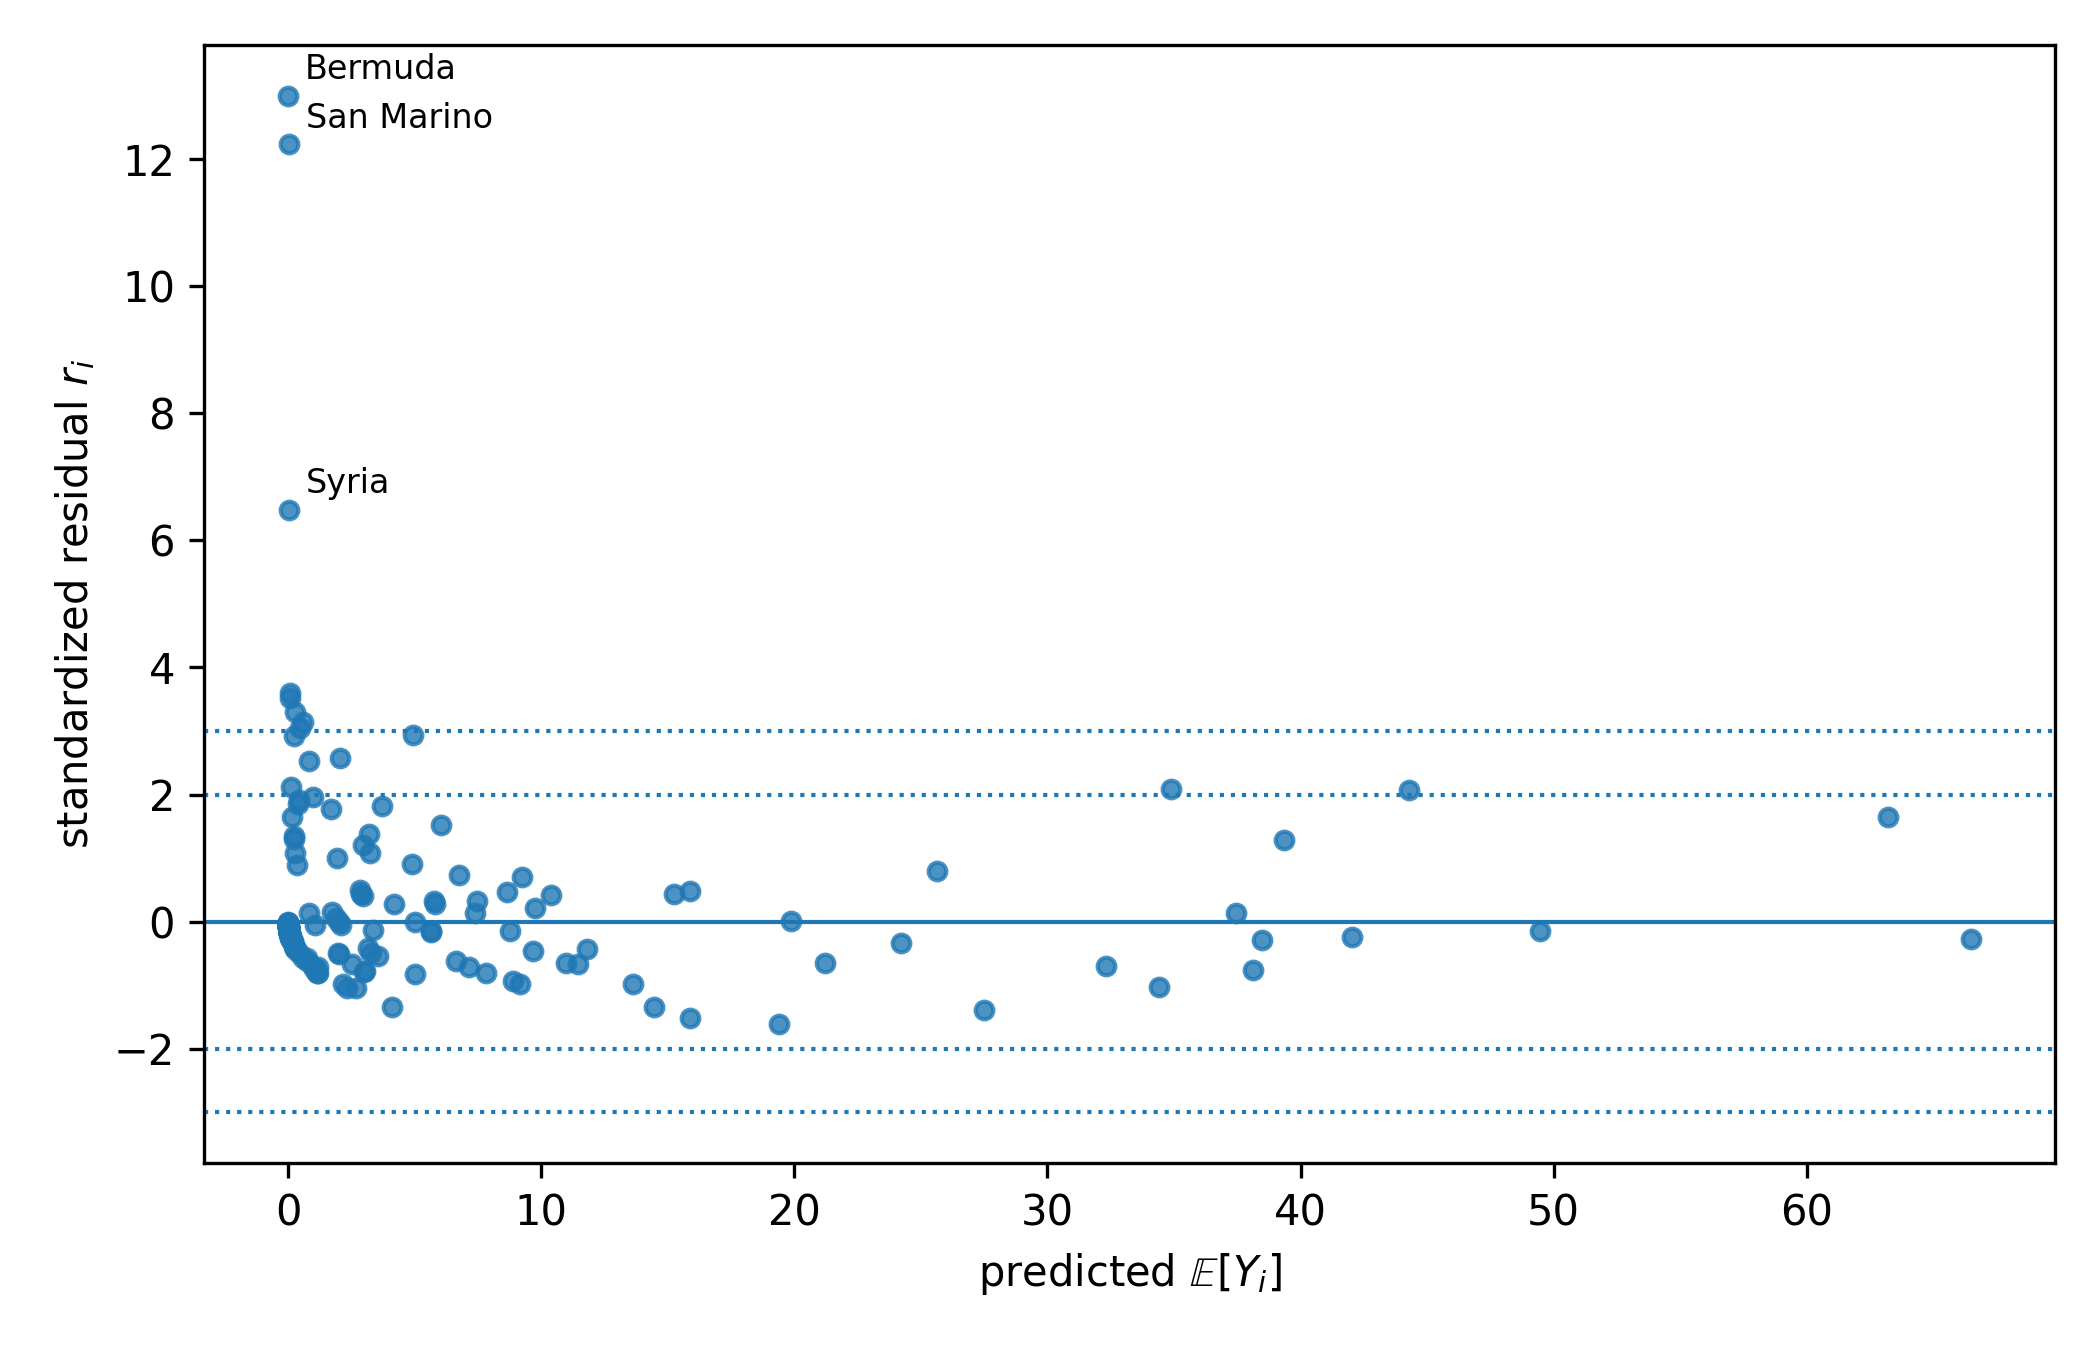
\includegraphics[width=0.92\linewidth]{fig_resid_vs_pred.png}
  \caption{Standardized residuals versus fitted means (ZINB).
  Notes: Points denote NOCs; horizontal lines mark $r_i=0$ and $r_i=\pm2,\pm3$; labels highlight the three countries with the largest residual rankings.}
  \label{fig:resid_vs_pred}
\end{figure}

Figure~\ref{fig:resid_vs_pred} examines how standardized residuals vary with the 
fitted means. In the mid-to-high fitted range ($\widehat{\mathbb{E}}[Y_i]>15$), 
points scatter randomly around zero with no visible curvature or fan-shaped spread, 
indicating no material bias or heteroskedasticity for major medal-winning NOCs. 
By contrast, the \emph{largest} deviations are concentrated at the \emph{low-fitted} 
end: when $\widehat{\mathbb{E}}[Y_i]\approx 0$, a few teams---notably 
\textbf{Bermuda}, \textbf{San Marino}, and \textbf{Syria}---exceed $r_i>3$, 
meaning that realized medals substantially surpass model expectations. 
These rare and low-baseline successes are precisely the horizontal manifestation
of the heavy right tail highlighted in Figure~\ref{fig:resid_hist}. 
Thus, while the ZINB specification addresses structural zeros and overdispersion, 
some upper-tail underprediction remains for a small set of low-baseline NOCs. 
Robustness checks will therefore incorporate covariates for rare successes 
(e.g., host-country indicator, event-mix or investment controls, per-capita/scale-normalized 
measures, and interactions with $\log(\mathrm{Athletes})$), and, if needed, 
hierarchical/random-effects extensions to target the low-fitted group.

\subsubsection{Predicted Medal Counts Against Key Covariates Under the ZINB Model}
\label{subsubsec:fourpanels-rev}

\begin{figure}[H]
  \centering
  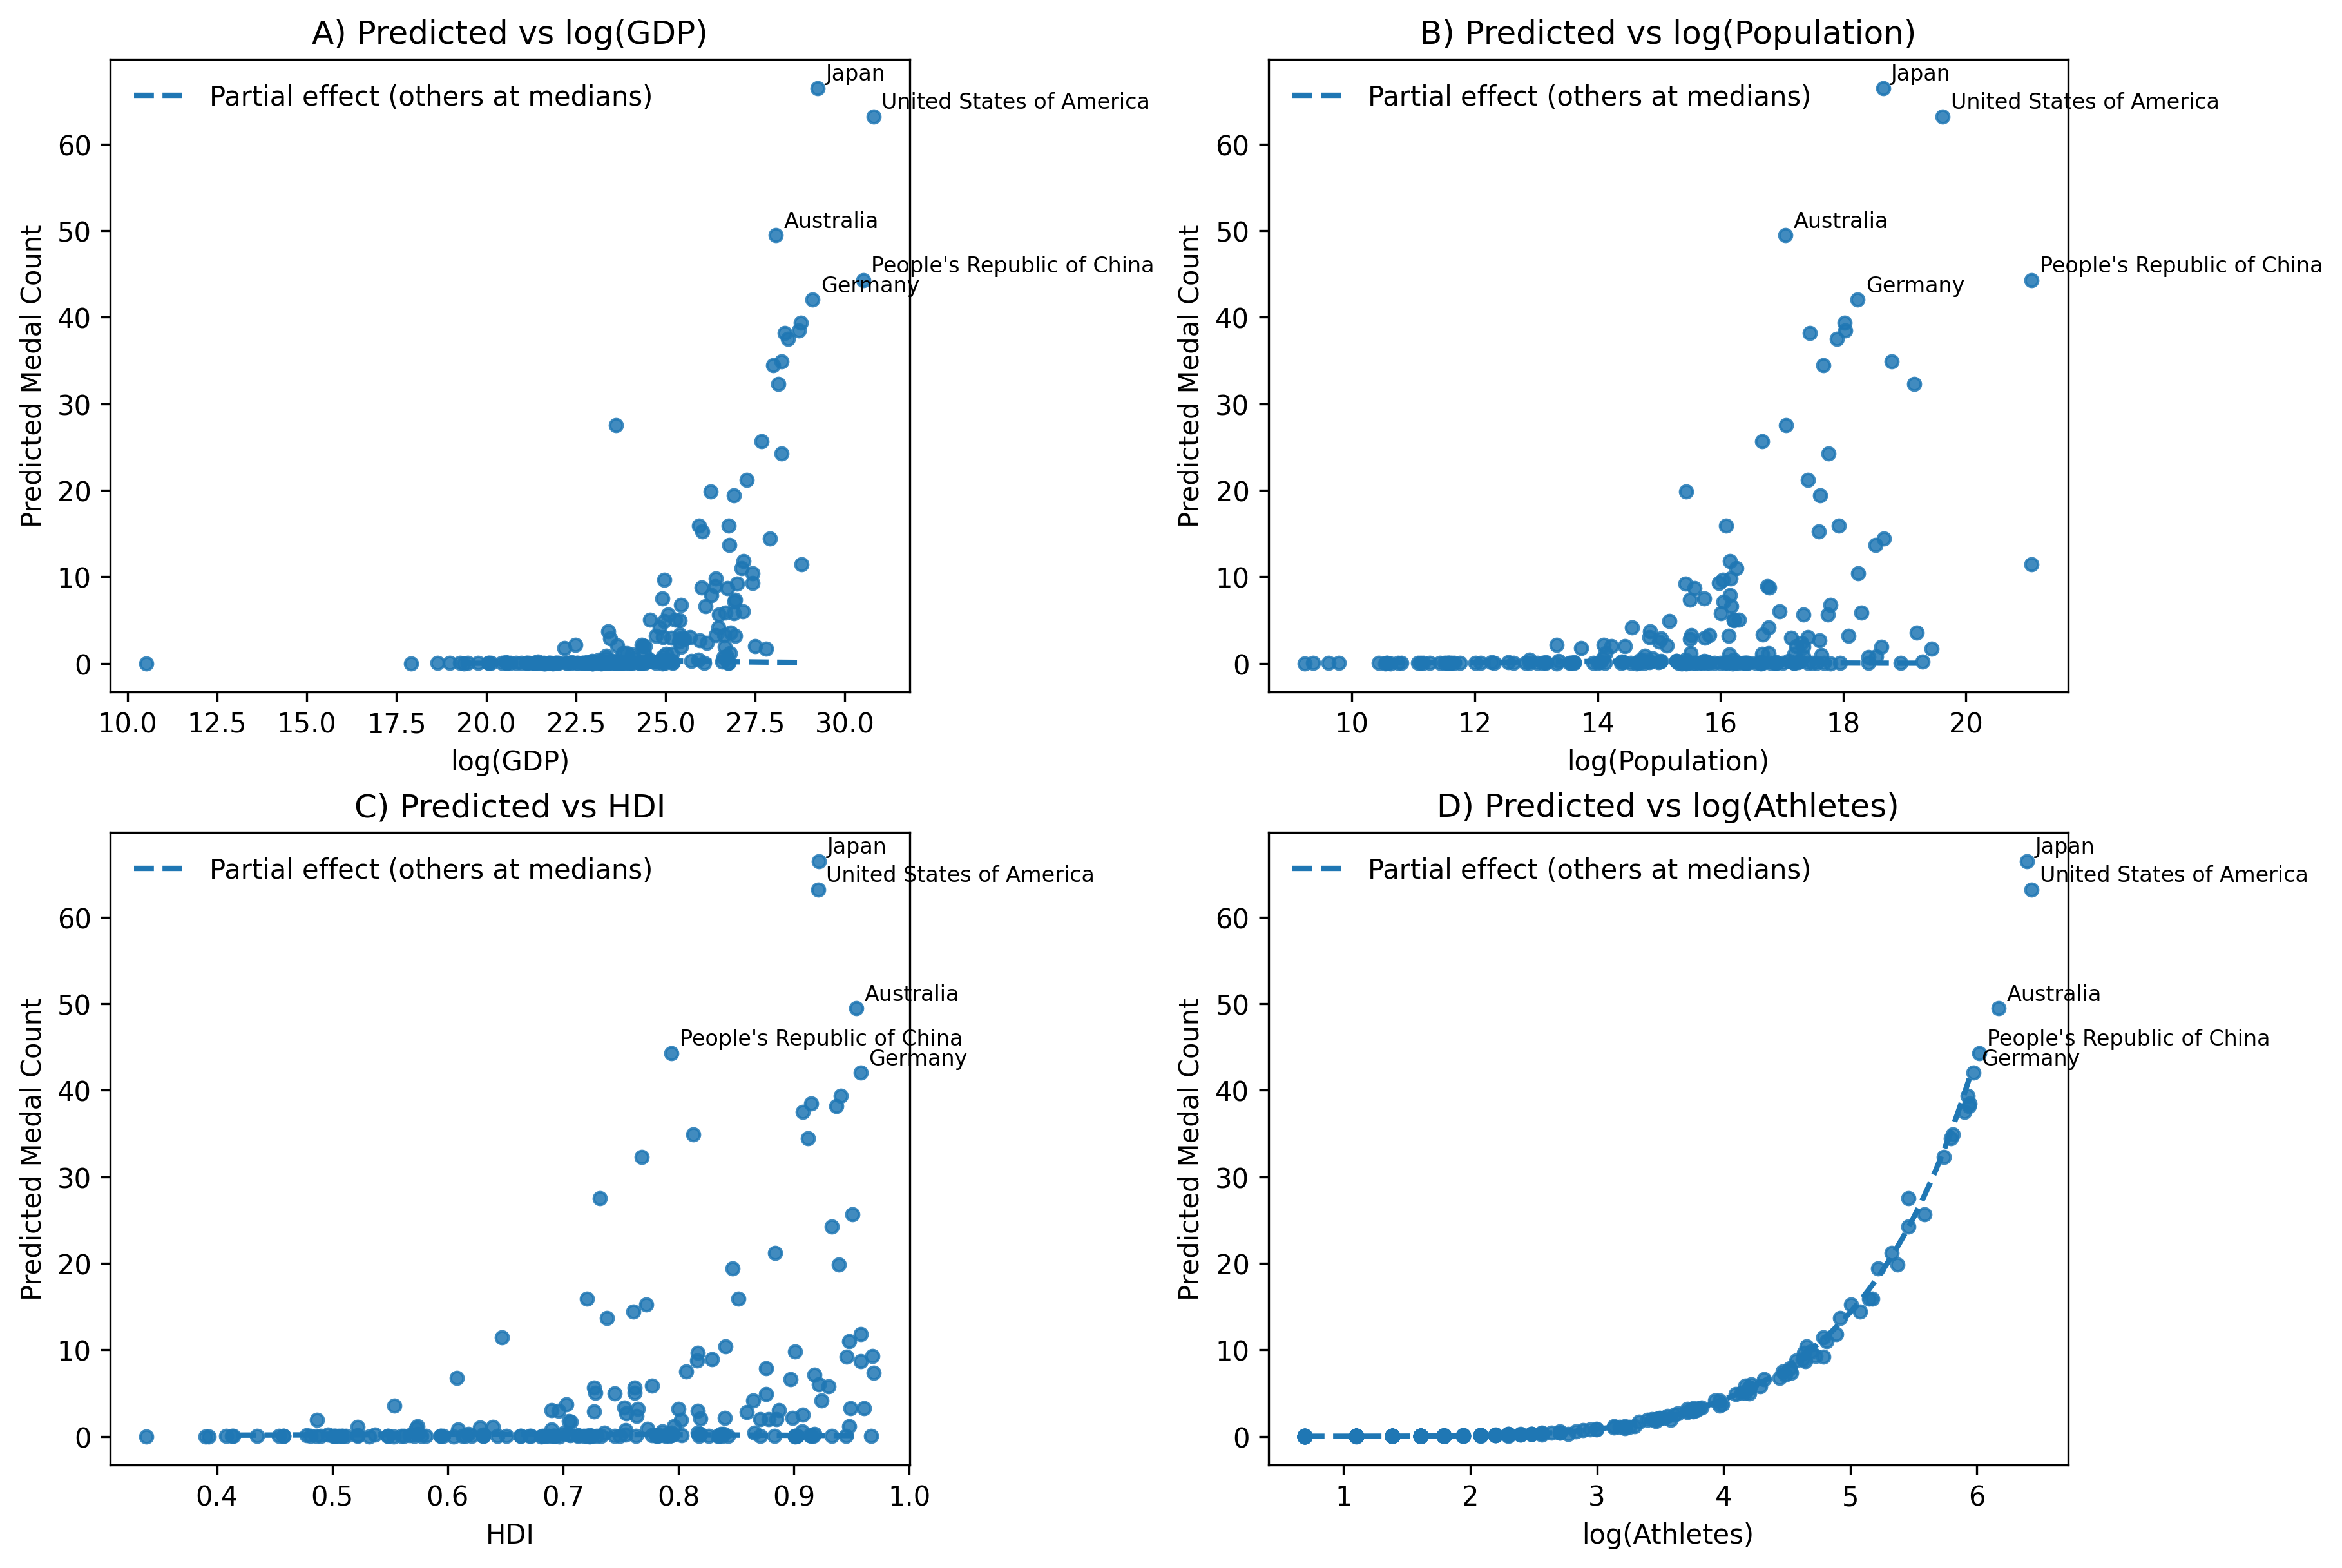
\includegraphics[width=\linewidth]{four_panels_zinb.png}
  \caption{Predicted medal counts versus key covariates under the ZINB model.
For panels (A)--(D), the horizontal axes are $\log(\mathrm{GDP})$,
$\log(\mathrm{Population})$, HDI (unlogged), and $\log(\mathrm{Athletes})$,
respectively; the vertical axis in all panels is the predicted expectation. Points denote individual NOCs
at their observed covariate values. The dashed curve in each panel is a
ceteris paribus partial-effect function obtained by varying only the focal
covariate (holding the others at their sample medians) and recomputing
$\widehat{E}[Y]$.}

  \label{fig:four-panels-zinb}
\end{figure}

As shown in Panel~A of Figure~\ref{fig:four-panels-zinb}, when Population, HDI, and the number of participating athletes are held at their medians, the ceteris paribus curve with respect to $\log(\mathrm{GDP})$ is nearly flat. This accords with the count coefficient $b_{\log GDP}=-0.18$ (n.s.). By contrast, the inflation part yields $\gamma_{\log GDP}<0$ (significant), indicating that GDP mainly lowers the probability of a structural zero---an entry-margin effect rather than a scale effect.

Panel~B of Figure~\ref{fig:four-panels-zinb} varies $\log(\mathrm{Population})$ while fixing the other covariates at their medians. The partial-effect curve rises only mildly, consistent with $c_{\log Pop}=0.20$ (n.s.), implying limited scale effects once participation is controlled for. The inflation estimate is positive and significant ($\gamma_{\log Pop}>0$), suggesting that, conditional on GDP, HDI, and athletes, more populous countries may still face a higher zero risk; Population is therefore not an effective proxy for participation.

Panel~C of Figure~\ref{fig:four-panels-zinb} considers HDI (unlogged). The curve increases with HDI but lacks statistical precision ($d_{\mathrm{HDI}}=1.93$, n.s.), consistent with HDI’s influence being mediated through channels already captured by participation and related inputs.

Panel~D of Figure~\ref{fig:four-panels-zinb} varies $\log(\mathrm{Athletes})$. The curve is steeply upward and matches the significant count estimate $e_{\log Ath}=1.10$: a 1\% increase in the number of participating athletes raises the expected medal count by about 1.10\%. Moreover, $\gamma_{\log Ath}<0$ (significant) shows that sending more athletes substantially reduces the structural-zero probability.

Across the Figure~\ref{fig:four-panels-zinb}, the number of participating athletes is the dominant driver of post-entry medal scale and also reduces the zero risk; GDP primarily improves the entry margin; Population adds little explanatory power once participation is controlled for; and the positive effect of HDI is not robust.


\subsection{Case Study of High Residual Countries}

This section further presents the comparison between the model predictions and the actual medal outcomes at the Tokyo 2020 Olympic Games. Several countries exhibited substantial deviations from the predicted values. Tables~\ref{tab:over} and \ref{tab:under} list the top five countries with significantly higher medal counts than predicted (Over-Performance) and those with significantly fewer medals than predicted (Under-Performance). The analysis of these cases highlights specific factors beyond the scope of macro-level explanatory variables, such as the decisive role of individual elite athletes, targeted sports policies, and cultural traditions.

\subsubsection{Analysis of Nations Overperforming Model Forecasts}

\begin{table}[H]
\centering
\caption{Top Five Over-Performing Countries}
\label{tab:over}
\begin{tabular}{ccc}
\hline
Country & Actual Medals & Predicted Medals \\
\hline
San Marino & 3 & 0.1 \\
Syria & 1 & 0.2 \\
Bermuda & 1 & 0.05 \\
Mongolia & 4 & 1.2 \\
Fiji & 2 & 0.4 \\
\hline
\end{tabular}
\end{table}

\textbf{San Marino} achieved a historic breakthrough at the Tokyo 2020 Olympics, winning three medals (one silver and two bronze), despite being the smallest country ever to reach the Olympic podium. Alessandra Perilli won bronze in women’s trap shooting, the first Olympic medal in San Marino’s history, and later secured a silver medal in the mixed team trap event. These achievements highlight the impact of a single elite athlete in niche sports, which macro-level models cannot fully anticipate \citep{gasquez2014}.  

\textbf{Syria}, despite facing prolonged conflict and economic hardship, secured a silver medal through weightlifter Man Asaad in the men’s 109kg+ category. This was only the second Olympic medal in Syria’s weightlifting history, underlining how the extraordinary performance of individual athletes can lead to outcomes far beyond model expectations \citep{Bernard2004}.  

\textbf{Bermuda}, with fewer than 100,000 inhabitants, won its first-ever Olympic gold medal in Tokyo. Flora Duffy’s victory in the women’s triathlon not only marked a historic achievement but also demonstrated how concentrated investment in a single sport can yield outsized returns for small nations \citep{hoffmann2002}.  

\textbf{Mongolia} continued its strong tradition in combat sports, earning four medals across judo and wrestling. Notably, Tsend-Ochir Tsogtbaatar won bronze in the men’s judo 73kg category. Mongolia’s cultural emphasis and targeted investment in martial arts explain its over-performance relative to the model’s prediction \citep{andreff2015}.  

\textbf{Fiji}, a small island nation, repeated its dominance in rugby sevens, winning gold in the men’s event and bronze in the women’s. Fiji’s reliance on a single team sport with world-class strength illustrates how collective excellence can propel a country far beyond statistical expectations \citep{darby2017}.  

\subsubsection{Analysis of Nations Underperforming Model Forecasts}

\begin{table}[H]
\centering
\caption{Top Five Under-Performing Countries}
\label{tab:under}
\begin{tabular}{ccc}
\hline
Country & Actual Medals & Predicted Medals \\
\hline
India & 7 & 17 \\
Nigeria & 2 & 6 \\
Egypt & 6 & 11 \\
South Africa & 3 & 8 \\
Mexico & 4 & 9 \\
\hline
\end{tabular}
\end{table}

\textbf{India}, despite its vast population and rising GDP, secured only 7 medals at Tokyo 2020, far below the predicted 17. Although Neeraj Chopra’s gold medal in men’s javelin throw was a historic achievement, India underperformed in shooting and wrestling, which had previously been strong areas. The dominance of cricket, a non-Olympic sport, also diverts talent and resources away from Olympic disciplines \citep{kaplanidou2010}.  

\textbf{Nigeria} won just 2 medals (in wrestling and athletics), compared to a predicted 6. Blessing Oborududu earned a silver in women’s wrestling, while Ese Brume took bronze in long jump. Yet, systemic challenges such as underfunding, administrative disorganization, and lack of infrastructure limit Nigeria’s Olympic potential \citep{amusa2003}.  

\textbf{Egypt} earned 6 medals, mostly in weightlifting and karate, compared to the predicted 11. While Feryal Abdelaziz’s gold in women’s karate marked a breakthrough, other traditional strengths like wrestling and weightlifting fell short, reflecting fluctuations in performance across Olympic cycles \citep{solberg2007}.  

\textbf{South Africa} managed only 3 medals (including Tatjana Schoenmaker’s gold and silver in swimming), well below the predicted 8. Despite strong traditions in swimming and athletics, political and economic transitions have constrained sports investment, limiting performance \citep{burnett2010}.  

\textbf{Mexico} earned 4 medals compared to a predicted 9. Although Mexico has historically performed well in boxing, taekwondo, and diving, its Tokyo performance was weaker than in London or Rio. The case illustrates that economic resources alone cannot guarantee Olympic success \citep{bellos2016}.  

\subsection{Heterogeneity Analysis}
\subsubsection{Heterogeneity Analysis by Population Size}

To further investigate the effect of population size on prediction bias, this section classifies NOCs into four categories: \textit{Small} (population below 10 million), \textit{Medium-Small} (10 to 50 million), \textit{Medium-Large} (50 to 100 million), and \textit{Large} (over 100 million). Table~\ref{tab:POP_groups_residuals} presents the prediction residuals across these groups.  

The results show that \textit{Small} countries have an average residual close to zero (0.024) and a median residual near zero (-0.012), suggesting overall accurate predictions. However, more than 90\% of small countries won fewer medals than predicted, indicating systematic overestimation by the model. For the \textit{Medium-Small} group, the mean residual is positive (0.565), with around 43\% of countries over-performing and 57\% under-performing relative to predictions, reflecting a relatively balanced distribution of errors. In contrast, the \textit{Medium-Large} group shows a negative mean residual (-0.455), implying that the model tends to underestimate this group’s medal counts. Yet nearly 78\% of countries in this group still underperformed relative to predictions, pointing to persistent overestimation bias. Finally, the \textit{Large} group exhibits the highest mean residual (0.828) and the largest standard deviation (12.447), indicating the most heterogeneous and unstable prediction errors. Overall, the findings highlight pronounced heterogeneity in model performance across population groups, with prediction bias being especially evident among small and large countries.  


\begin{table}[htbp]
\centering
\caption{Prediction residuals by population-size groups}
\label{tab:POP_groups_residuals}
\resizebox{\textwidth}{!}{%
\begin{tabular}{ccccccc}
\toprule
\textbf{Pop. Group} & \textbf{N} & \textbf{Mean Residual} & \textbf{Median Residual} & \textbf{SD Residual} & \textbf{Share Over-Perf.} & \textbf{Share Under-Perf.} \\
\midrule
Small         & 52 & 0.024 & -0.012 & 0.622  & 0.096 & 0.904 \\
Medium-Small  & 51 & 0.565 & -0.002 & 1.759  & 0.431 & 0.569 \\
Medium-Large  & 51 & -0.455 & -0.025 & 4.840 & 0.216 & 0.784 \\
Large         & 52 & 0.828 & -0.059 & 12.447 & 0.308 & 0.692 \\
\bottomrule
\end{tabular}}
\par\vspace{6pt}
\begin{minipage}{0.95\linewidth}
\footnotesize
\raggedright
\textit{Notes:} Residual is defined as \textbf{Actual -- Predicted}; a positive value means the model under-predicted medal counts, while a negative value indicates over-prediction. 
SD Residual measures the dispersion of residuals within each population group, where larger values imply greater heterogeneity in prediction errors. 
\textbf{Share Over-Perf.} and \textbf{Share Under-Perf.} present the proportions of countries within each group with residuals greater than zero (actual $>$ predicted) or less than zero (actual $<$ predicted), respectively.
\end{minipage}
\end{table}


\subsubsection{Heterogeneity Analysis by GDP Levels}

In the heterogeneity analysis based on GDP levels, the sample countries are divided into four quartile groups according to per capita GDP: \textbf{Low income, Lower-middle income, Upper-middle income, and High income}. The results, as shown in Table~\ref{tab:gdp_groups_residuals}, indicate that there are significant differences in prediction bias across groups. Low-income countries have an average residual close to zero, indicating overall accurate predictions, but more than 90\% of countries fall below the predicted medal counts, with only a small fraction over-performing. Lower-middle income countries exhibit a negative mean residual, showing slightly fewer medals than predicted, while internal variation is substantial, with only about one quarter of countries exceeding predictions and most under-performing.  

In the upper-middle income group, the mean residual turns positive, suggesting that overall medal counts are higher than predicted, but internal disparities remain evident, with just over one third of countries showing over-performance. High-income countries also record a positive mean residual, but the variation of residuals is the largest, indicating strong internal heterogeneity: about one third of countries exceed predictions, while the majority fall short. Overall, as GDP level increases, the dispersion of prediction residuals becomes more pronounced, implying that although economic strength is an important factor, it is not the sole determinant of Olympic medal performance, with sports tradition, policy support, and competitive advantages also playing crucial roles.


\begin{table}[H]
\centering
\caption{Prediction residuals by GDP groups}
\label{tab:gdp_groups_residuals}
\resizebox{\textwidth}{!}{%
\begin{tabular}{ccccccc}
\hline
\textbf{GDP Group} & \textbf{N} & \textbf{Mean Residual} & \textbf{Median Residual} & \textbf{SD Residual} & \textbf{Share Over-Perf.} & \textbf{Share Under-Perf.} \\
\hline
Low GDP & 52 & 0.036 & -0.006 & 0.549  & 0.077 & 0.923 \\
Lower-Middle GDP & 51 & -0.126 & -0.011 & 4.129  & 0.255 & 0.745 \\
Upper-Middle GDP & 51 & 0.528  & -0.016 & 2.146  & 0.353 & 0.647 \\
High GDP & 52 & 0.529  & -1.145 & 12.666 & 0.365 & 0.635 \\
\hline
\end{tabular}%
}
\vspace{0.3em}
\begin{flushleft}
\footnotesize
\textit{Notes}: Definitions of residuals and performance shares are the same as in Table~\ref{tab:POP_groups_residuals}.
\end{flushleft}
\end{table}

\subsubsection{Heterogeneity Analysis by Athlete Size}

In the heterogeneity analysis based on the number of participating athletes, countries were divided into four groups according to the quartiles of athlete size: \textbf{Small}, \textbf{Medium-Small}, \textbf{Medium-Large}, and \textbf{Large}. As shown in Table~\ref{tab:ath_groups_residuals}, clear differences emerge across groups. For Small and Medium-Small countries, the mean residuals are close to zero (0.047 and 0.084, respectively), and the median residuals are nearly zero as well, suggesting overall accurate predictions. However, more than 80\% of countries in these groups actually underperformed relative to model expectations (97.0\% and 83.3\%), indicating systematic under-performance. For Medium-Large countries, the mean residual rises to 0.319, and 45.1\% of countries exceed their predicted medal counts, suggesting stronger underestimation by the model. The Large group shows a higher mean residual (0.529) but a notably negative median residual (-0.714), reflecting substantial within-group heterogeneity. In this group, 44.2\% of countries outperform predictions while 55.8\% underperform, and the standard deviation of residuals (13.344) is far larger than in other groups. These results highlight that prediction errors become more volatile with larger athlete delegations, posing greater challenges for the model in capturing the performance of the largest teams.

\begin{table}[H]
\centering
\caption{Prediction residuals by athlete-size groups}
\label{tab:ath_groups_residuals}
\resizebox{\textwidth}{!}{%
\begin{tabular}{ccccccc}
\toprule
\textbf{Athlete Group} & \textbf{N} & \textbf{Mean Residual} & \textbf{Median Residual} & \textbf{SD Residual} & \textbf{Share Over-Perf.} & \textbf{Share Under-Perf.} \\
\midrule
Small         & 67 & 0.047 & -0.006 & 0.381  & 0.030 & 0.970 \\
Medium-Small  & 36 & 0.084 & -0.057 & 0.372  & 0.167 & 0.833 \\
Medium-Large  & 51 & 0.319 & -0.090 & 1.966  & 0.451 & 0.549 \\
Large         & 52 & 0.529 & -0.714 & 13.344 & 0.442 & 0.558 \\
\bottomrule
\end{tabular}}
\par\vspace{6pt}
\begin{minipage}{0.95\linewidth}
\raggedright
\footnotesize
\textit{Notes}: Definitions of residuals and performance shares are the same as in Table~\ref{tab:POP_groups_residuals}.
\end{minipage}
\end{table}


\subsubsection{Heterogeneity Analysis by HDI Levels}

In the heterogeneity analysis based on HDI levels, countries were divided into four groups according to the quartiles of the Human Development Index: \textbf{Low HDI}, \textbf{Lower-Middle HDI}, \textbf{Upper-Middle HDI}, and \textbf{High HDI}. As shown in Table~\ref{tab:hdi_groups_residuals}, different groups exhibit distinct patterns of prediction residuals. The Low HDI group displays residuals close to zero on average, with a mean of 0.101 and a median of -0.007, suggesting that the model's predictions broadly align with actual medal counts. However, nearly 89\% of the countries in this group underperformed relative to the predictions, indicating systematic difficulties in achieving expected results. The Lower-Middle HDI group shows a negative mean residual of -0.592, reflecting a tendency of over-prediction, though about three-quarters of the countries still underperformed. In contrast, the Upper-Middle HDI group presents a substantially positive mean residual of 1.081, with nearly 37\% of countries over-performing, highlighting stronger-than-expected outcomes. Finally, the High HDI group reveals a positive mean residual of 0.380, but also the largest dispersion (SD = 8.955), suggesting high variability: while roughly one-third of these countries exceed model expectations, a similar proportion fall short. This pattern indicates that higher human development is generally associated with stronger performance, yet it also brings greater heterogeneity in Olympic outcomes, shaped by additional factors such as institutional support, sports culture, and national investment.


\begin{table}[htbp]
\centering
\caption{Prediction residuals by HDI groups}
\resizebox{\textwidth}{!}{%
\begin{tabular}{ccccccc}
\toprule
\textbf{HDI Group} & \textbf{N} & \textbf{Mean Residual} & \textbf{Median Residual} & \textbf{SD Residual} & \textbf{Share Over-Perf.} & \textbf{Share Under-Perf.} \\
\midrule
Low HDI          & 52 & 0.101  & -0.007 & 0.786  & 0.115 & 0.885 \\
Lower-Middle HDI & 51 & -0.592 & -0.011 & 4.822  & 0.235 & 0.765 \\
Upper-Middle HDI & 51 & 1.081  & -0.035 & 8.877  & 0.373 & 0.627 \\
High HDI         & 52 & 0.380  & -0.054 & 8.955  & 0.327 & 0.673 \\
\bottomrule
\end{tabular}}
\par\vspace{6pt}
\begin{minipage}{0.95\linewidth}
\footnotesize
\raggedright
\footnotesize
\textit{Notes}: Definitions of residuals and performance shares are the same as in Table~\ref{tab:POP_groups_residuals}.
\end{minipage}
\end{table}


\section{Robustness and Sensitivity Analyses}
\subsection{Comparison with Alternative Models}

To provide a more comprehensive assessment of model performance, this section compares the Zero-Inflated Negative Binomial (ZINB) model with three models: the standard Poisson regression, the Negative Binomial regression (NB2), and the Zero-Inflated Poisson (ZIP). All models were estimated using the same set of explanatory variables, namely log-transformed GDP, log-transformed population, Human Development Index (HDI), and log-transformed number of athletes. For the zero-inflated models, the inflation component employed the same covariates with a logit link function to account for excess zeros. All estimations were carried out in Python using the \texttt{statsmodels} package under the maximum likelihood framework, and model fit was evaluated based on log-likelihood, AIC, BIC, and pseudo-$R^2$ statistics. However, the explanatory power of Pseudo-$R^2$ is limited in count data models, and its values are not as straightforwardly interpretable as in linear regression. Therefore, this study mainly relies on the log-likelihood, AIC, and BIC as the primary criteria for comparing model performance.



Table \ref{tab:model_comparison} shows the comparative model fit statistics for the Poisson, Negative Binomial (NB2), Zero-Inflated Poisson (ZIP), and Zero-Inflated Negative Binomial (ZINB) specifications. Among the four models, the ZINB achieves the lowest AIC and BIC values, indicating the best overall fit. This finding confirms the presence of both overdispersion (as captured by the significant dispersion parameter $\alpha$) and excess zeros in the medal count data, making the ZINB model more suitable than its simpler alternatives. While the standard Poisson and ZIP models exhibit substantially higher AIC/BIC, suggesting poorer fit, the NB2 model provides an improvement over Poisson but still underperforms relative to ZINB.

\begin{table}[H]
\centering
\caption{Model comparison across Poisson, NB2, ZIP, and ZINB.}
\label{tab:model_comparison}
\begin{tabular}{cccccc}
\toprule
Model & Converged & LogLik & AIC & BIC & alpha \\
\midrule
ZINB (Zero-Inflated NB2)   & True & -294.103 & 610.206 & 646.812 & 0.215 \\
NB2 (Negative Binomial)    & True & -305.311 & 622.621 & 642.589 & 0.331 \\
ZIP (Zero-Inflated Poisson)& True & -343.019 & 706.037 & 739.316 &      NaN\\
Poisson (GLM)              & True & -362.901 & 735.801 & -674.495 &      NaN\\
\bottomrule
\end{tabular}
\end{table}

It is important to note that the Poisson and ZIP models do not estimate an overdispersion parameter, which explains why the value of $\alpha$ is not applicable (NaN). In these specifications, the variance is constrained to equal the mean, consistent with the standard Poisson assumption. By contrast, both the NB2 and ZINB models relax this restriction by introducing an additional dispersion parameter $\alpha$, where $\text{Var}(Y) = \mu + \alpha \mu^2$. The significantly positive estimates of $\alpha$ in NB2 and ZINB confirm the presence of overdispersion in the Olympic medal count data, reinforcing the appropriateness of adopting a negative binomial framework over the simpler Poisson-based alternatives.

\subsection{Sensitivity Analysis with Alternative Covariates}

To assess the robustness of the main findings, this study further examined whether the results are sensitive to alternative covariate specifications. Specifically, a series of Zero-Inflated Negative Binomial (ZINB) regressions were re-estimated by either excluding one of the main explanatory variables (GDP, HDI, or population) or by using a simplified specification that only includes GDP and the number of athletes. The purpose of this exercise is to verify whether the key conclusions rely heavily on a specific variable, or whether they remain stable across different model settings.

Table~\ref{tab:zinb_alt_specs} shows the model fit statistics across these alternative specifications. The results indicate that all models converge successfully, with relatively similar log-likelihood, AIC, and BIC values. Notably, the ``Drop HDI'' and ``Drop Population'' specifications yield slightly lower AIC and BIC than the full model, suggesting marginal improvements in fit, while the ``GDP + Athletes only'' model also performs comparably well. The dispersion parameter $\alpha$ remains positive across all specifications, confirming the presence of overdispersion and validating the use of the ZINB framework.

\begin{table}[H]
\centering
\caption{Model comparison across alternative ZINB specifications}
\label{tab:zinb_alt_specs}
\begin{tabular}{cccccc}
\hline
Model              & Converged & LogLik   & AIC     & BIC     & alpha \\
\hline
Drop HDI           & True      & -292.929 & 603.857 & 633.808 & 0.250 \\
Drop Population    & True      & -295.405 & 608.809 & 638.760 & 0.250 \\
GDP + Athletes only& True      & -298.021 & 610.042 & 633.337 & 0.213 \\
Full model         & True      & -294.103 & 610.206 & 646.812 & 0.215 \\
Drop GDP           & True      & -296.941 & 611.882 & 641.833 & 0.209 \\
\hline
\end{tabular}
\end{table}

Table~\ref{tab:zinb_alt_specs_irr} presents the incidence rate ratios (IRR) of the main explanatory variables across the different specifications. The results show that the coefficient for \texttt{log\_Athletes} is consistently positive, statistically significant, and of similar magnitude across all models, reinforcing its strong predictive power for medal counts. The effects of \texttt{log\_GDP}, \texttt{log\_Pop}, and HDI vary somewhat across specifications, but the qualitative patterns remain broadly consistent. This robustness check therefore strengthens the conclusion that the number of athletes is the most reliable predictor of Olympic medal performance.

\begin{table}[H]
\centering
\caption{Count-part IRR (exp(coef)) across alternative ZINB specifications}
\label{tab:zinb_alt_specs_irr}
\begin{tabular}{cccccc}
\hline
Term           & Drop GDP & Drop HDI & Drop Population & Full model & GDP + Athletes only \\
\hline
HDI            & 1.243    & NaN      & 1.114           & 6.170      & NaN  \\
Intercept      & 0.033    & 0.090    & 0.080           & 0.050      & 0.059 \\
log\_Athletes  & 2.902    & 3.668    & 3.657           & 3.042      & 3.058 \\
log\_GDP       & NaN      & 0.940    & 0.948           & 0.835      & 0.995 \\
log\_Pop       & 1.031    & 1.012    & NaN             & 1.216      & NaN  \\
\hline
\end{tabular}
\end{table}

Overall, the robustness checks demonstrate that the main conclusions are not driven by any single covariate. While GDP, population, and HDI show some variability depending on specification, the number of athletes consistently exerts a stable and significant effect on Olympic medal counts, underscoring its role as the most important determinant in the analysis.


\subsection{Subsample Robustness Analysis}

To further evaluate the robustness of the baseline specification, four subsample regressions were implemented: the full sample ($n=206$), a sample excluding the top three medal-winning nations ($n=203$), a sample excluding the bottom 25\% of countries by athlete participation ($n=139$), and a sample excluding all zero-medal nations ($n=93$). The first three subsamples were estimated using zero-inflated negative binomial (ZINB) models, while the ``Drop zero-medal nations'' subsample was estimated with a standard negative binomial model (NB2), since structural zeros are no longer present and an explicit inflation process is unnecessary.  

Table~\ref{tab:subsample_robustness} reports model diagnostics including log-likelihood, AIC, BIC, root mean squared error (RMSE), dispersion parameter ($\alpha$), and the inflation intercept where applicable. The results indicate strong consistency across specifications in terms of coefficient signs and magnitudes, but also highlight meaningful differences in fit and dispersion across subsamples. The NB2 specification for the nonzero subsample delivers the lowest AIC (508.19 compared to 615.01 for the full-sample ZINB), confirming that once structural zeros are removed, a simple count distribution suffices. The increase in RMSE (9.82 versus 6.52) reflects greater heterogeneity in predicting positive counts, but the absence of zero inflation nonetheless improves overall model parsimony.  

In contrast, for samples containing zeros, ZINB proves necessary. Excluding the top three countries substantially improves model fit (AIC $\approx$ 574.96), lowers RMSE (4.21), and reduces over-dispersion ($\alpha \approx 0.148$), indicating that extreme medal powers inflate dispersion and mask the underlying inflation mechanism. Removing small countries also improves AIC (584.10), yet increases both RMSE (7.89) and $\alpha$ (0.234), suggesting that heterogeneity is more pronounced among mid-sized nations rather than the smallest ones.  

Taken together, the subsample regressions confirm the robustness of the baseline findings. The central relationships between explanatory variables and medal counts remain stable, while the variations in fit indices highlight the contexts in which zero inflation is essential. Specifically, when zeros are abundant, ZINB provides superior fit; when zeros are eliminated, NB2 offers a more parsimonious and equally valid alternative. These results strengthen the credibility of the main conclusions by demonstrating their resilience under different sample compositions.  


\begin{table}[htbp]
\centering
\caption{Subsample robustness checks with ZINB and NB2 models}
\label{tab:subsample_robustness}
\resizebox{\textwidth}{!}{%
\begin{tabular}{ccccccccc}
\hline
\textbf{Subset} & \textbf{Model} & \textbf{$n$} & \textbf{LogLik} & \textbf{AIC} & \textbf{BIC} & \textbf{RMSE} & \textbf{$\alpha$} & \textbf{Inflate Intercept} \\
\hline
Drop zero-medal nations & NB2  &  93 & -248.095 & 508.190 & 523.386 & 9.816 & 0.189 & -- \\
Drop top 3 medal countries & ZINB & 203 & -276.479 & 574.958 & 611.403 & 4.213 & 0.148 & 0.855 \\
Drop small (bottom 25\% by Athletes) & ZINB & 139 & -281.048 & 584.097 & 616.376 & 7.890 & 0.234 & 0.588 \\
Full sample & ZINB & 206 & -296.505 & 615.009 & 651.616 & 6.524 & 0.218 & 0.514 \\
\hline
\end{tabular}%
}
\end{table}


\subsection{Visualization of Model Fit and Interaction Effects}

As shown in Table~\ref{tab:zinb_interactions}, the inclusion of interaction terms marginally improves predictive accuracy but does not surpass the baseline model in overall explanatory power. These findings can be further understood by considering the empirical distribution of Olympic medals.  

\begin{table}[H]
\centering
\caption{ZINB model comparison with interaction terms}
\label{tab:zinb_interactions}
\begin{tabular}{cccccc}
\hline
Model & LogLik & AIC & BIC & RMSE & $\alpha$ \\
\hline
Baseline (no interactions) & -296.50 & \textbf{615.01} & 651.62 & 6.52 & 0.218 \\
Add GDP $\times$ Pop & -295.73 & 615.45 & 655.39 & 5.54 & 0.186 \\
Add Athletes $\times$ HDI & -297.80 & 619.60 & 659.54 & 6.26 & 0.238 \\
Add both interactions & -296.07 & 618.14 & 661.41 & \textbf{5.36} & 0.209 \\
\hline
\end{tabular}
\end{table}

First, the GDP $\times$ Population interaction is virtually null (IRR$\approx$1.01), indicating that even for countries with both large economies and populations, such as the United States and China, the medal advantage is not driven by a multiplicative effect of size and wealth. Instead, their dominance stems from institutionalized investment in sports infrastructure and long-term athlete development systems. This explains why the GDP-population interaction does not yield significant improvements in model fit.  

Second, the negative Athletes $\times$ HDI interaction (IRR$\approx$0.49) is of greater substantive importance. In high-HDI countries such as Norway, Germany, or the United Kingdom, increasing delegation size does not translate proportionally into more medals. This reflects the "elite sport" characteristic, whereby success depends on efficiency, advanced training technologies, and talent specialization rather than sheer numbers. By contrast, in middle-HDI nations such as Brazil or Russia, the size of the delegation remains more strongly correlated with medal output.  

Finally, the combined interaction model achieves the lowest RMSE but higher AIC and BIC, suggesting that its predictive gains may be due to mild overfitting rather than substantive explanatory improvements. This highlights an important methodological implication: more complex models are not necessarily more insightful. Accordingly, the baseline specification is retained as the primary explanatory model, while interaction models are presented as robustness checks. In particular, the Athletes $\times$ HDI interaction provides useful supplementary evidence on how the marginal returns to delegation size diminish in highly developed contexts, enriching our understanding of global disparities in Olympic success.

To complement the results in Table~\ref{tab:zinb_interactions}, three visualizations are provided. Figure~\ref{fig:actual_pred} evaluates overall fit, whereas Figures~\ref{fig:ath_hdi} and \ref{fig:gdp_pop} illustrate the interaction patterns of Delegation Size $\times$ HDI and GDP $\times$ Population, respectively.

\textbf{Figure~\ref{fig:actual_pred} (Actual vs Predicted medals)} shows that most observations cluster around the $45^\circ$ line, indicating that the baseline ZINB model captures the aggregate pattern well. A higher dispersion is visible in the upper-right (large medal totals) and lower-left (small medal totals) corners, which is consistent with the RMSE patterns reported in Table~\ref{tab:zinb_interactions}: interaction specifications slightly improve prediction error while not necessarily reducing AIC/BIC.

\begin{figure}[H]
  \centering
  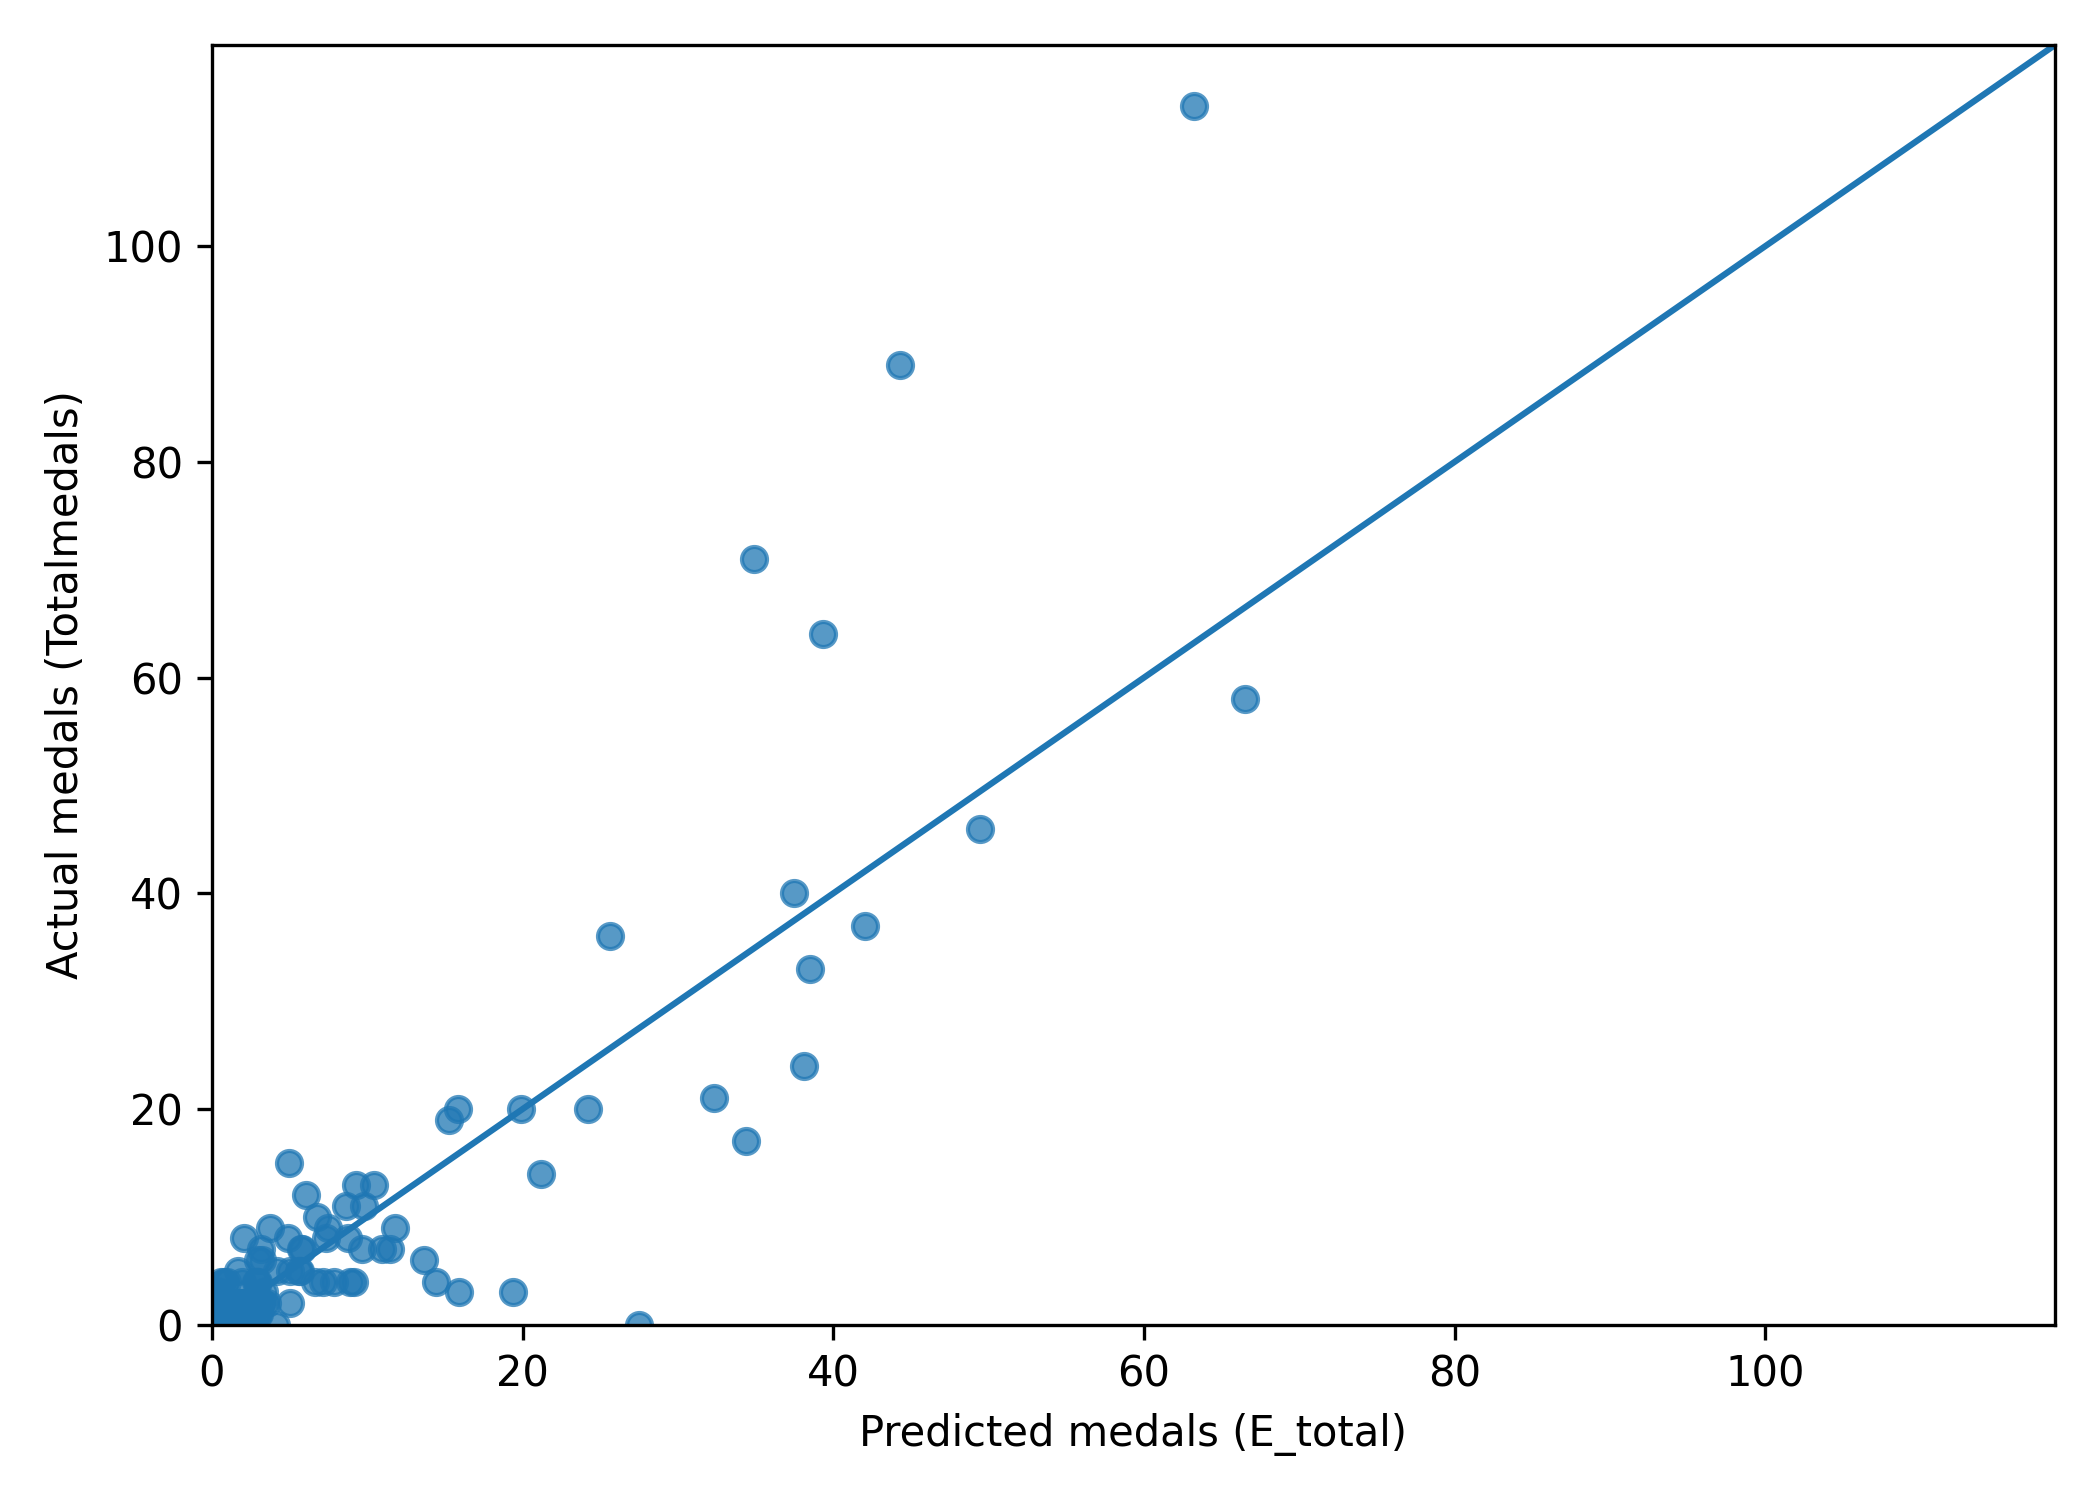
\includegraphics[width=0.75\textwidth]{fig_actual_vs_pred.png}
  \caption{Actual vs Predicted medals under the ZINB model}
  \label{fig:actual_pred}
\end{figure}

\textbf{Figure~\ref{fig:ath_hdi} (Delegation Size $\times$ HDI)} bins countries into HDI terciles (low/middle/high) and plots median medals across quantile bins of $\log(\text{Athletes})$. The curves for low and middle HDI groups rise more steeply with team size, whereas the high-HDI curve is markedly flatter. This aligns with the \emph{negative} Athletes $\times$ HDI interaction found in Table~\ref{tab:zinb_interactions} (e.g., IRR $\approx 0.49$ in the single-interaction model and $\approx 0.79$ in the combined model), implying diminishing marginal returns to delegation size in highly developed contexts.

\begin{figure}[H]
  \centering
  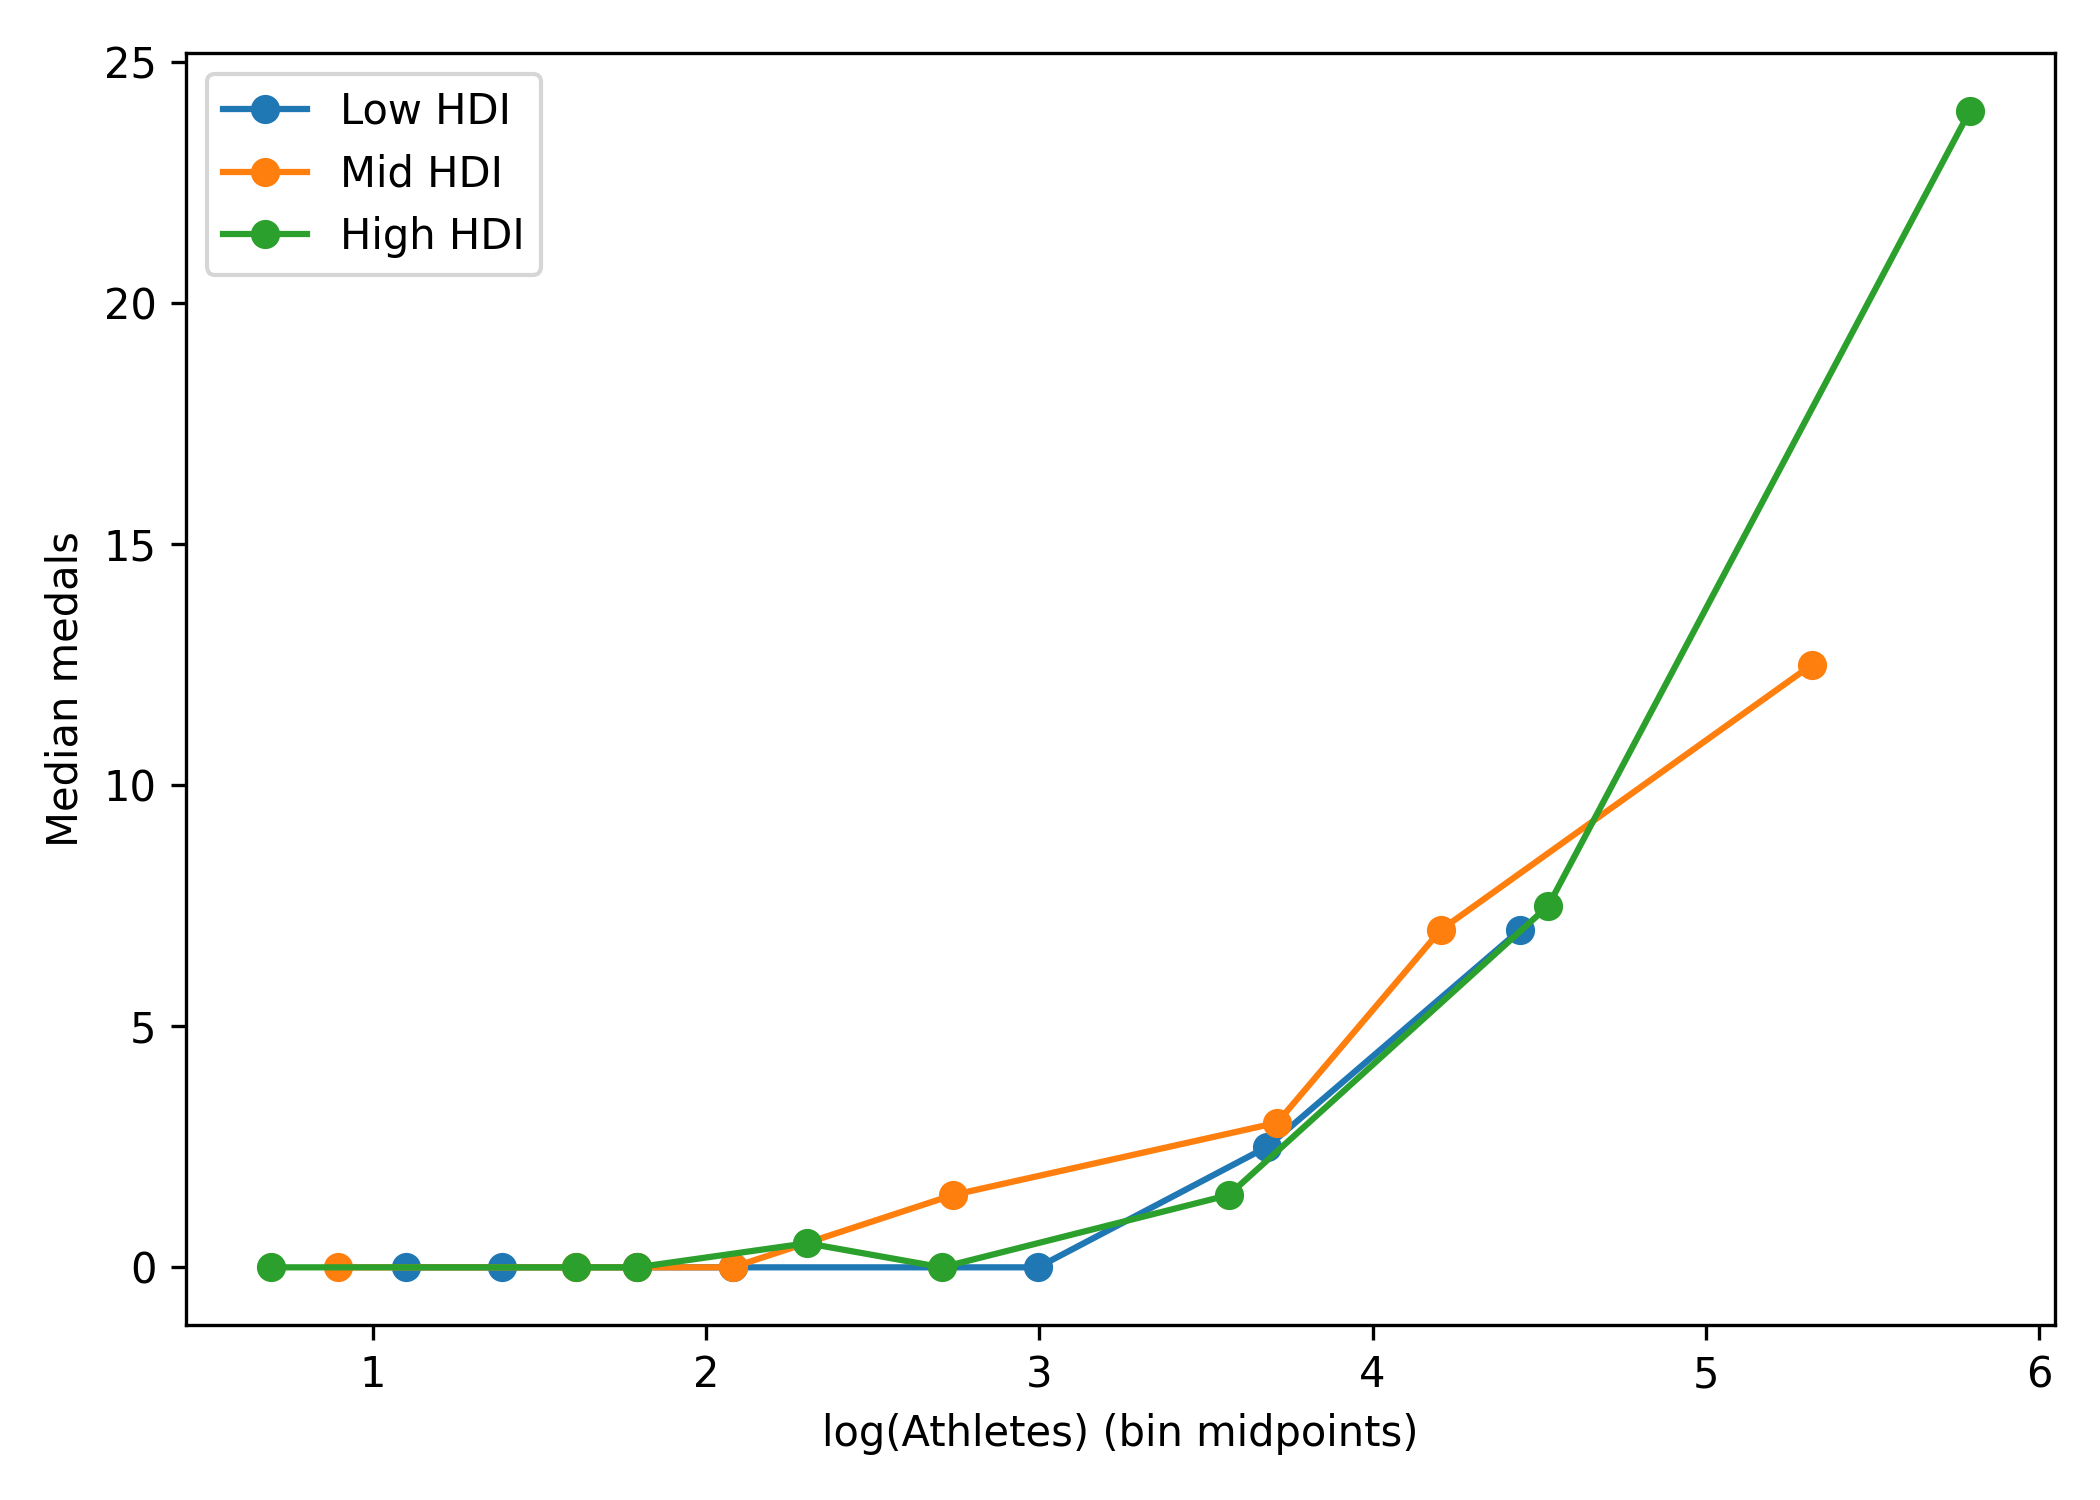
\includegraphics[width=0.75\textwidth]{fig_interaction_athletes_hdi.png}
  \caption{Interaction pattern: Delegation Size $\times$ HDI (binned medians)}
  \label{fig:ath_hdi}
\end{figure}


\textbf{Figure~\ref{fig:gdp_pop} (GDP $\times$ Population)} partitions countries into population quartiles and plots median medals across GDP bins. All curves increase with GDP, yet their slopes are broadly similar across population groups. The lack of clear separation is consistent with the near-zero GDP $\times$ Population interaction (IRR $\approx 1.01$) reported in Table~\ref{tab:zinb_interactions}, suggesting no meaningful multiplicative amplification between GDP and population beyond their main effects.

\begin{figure}[H]
  \centering
  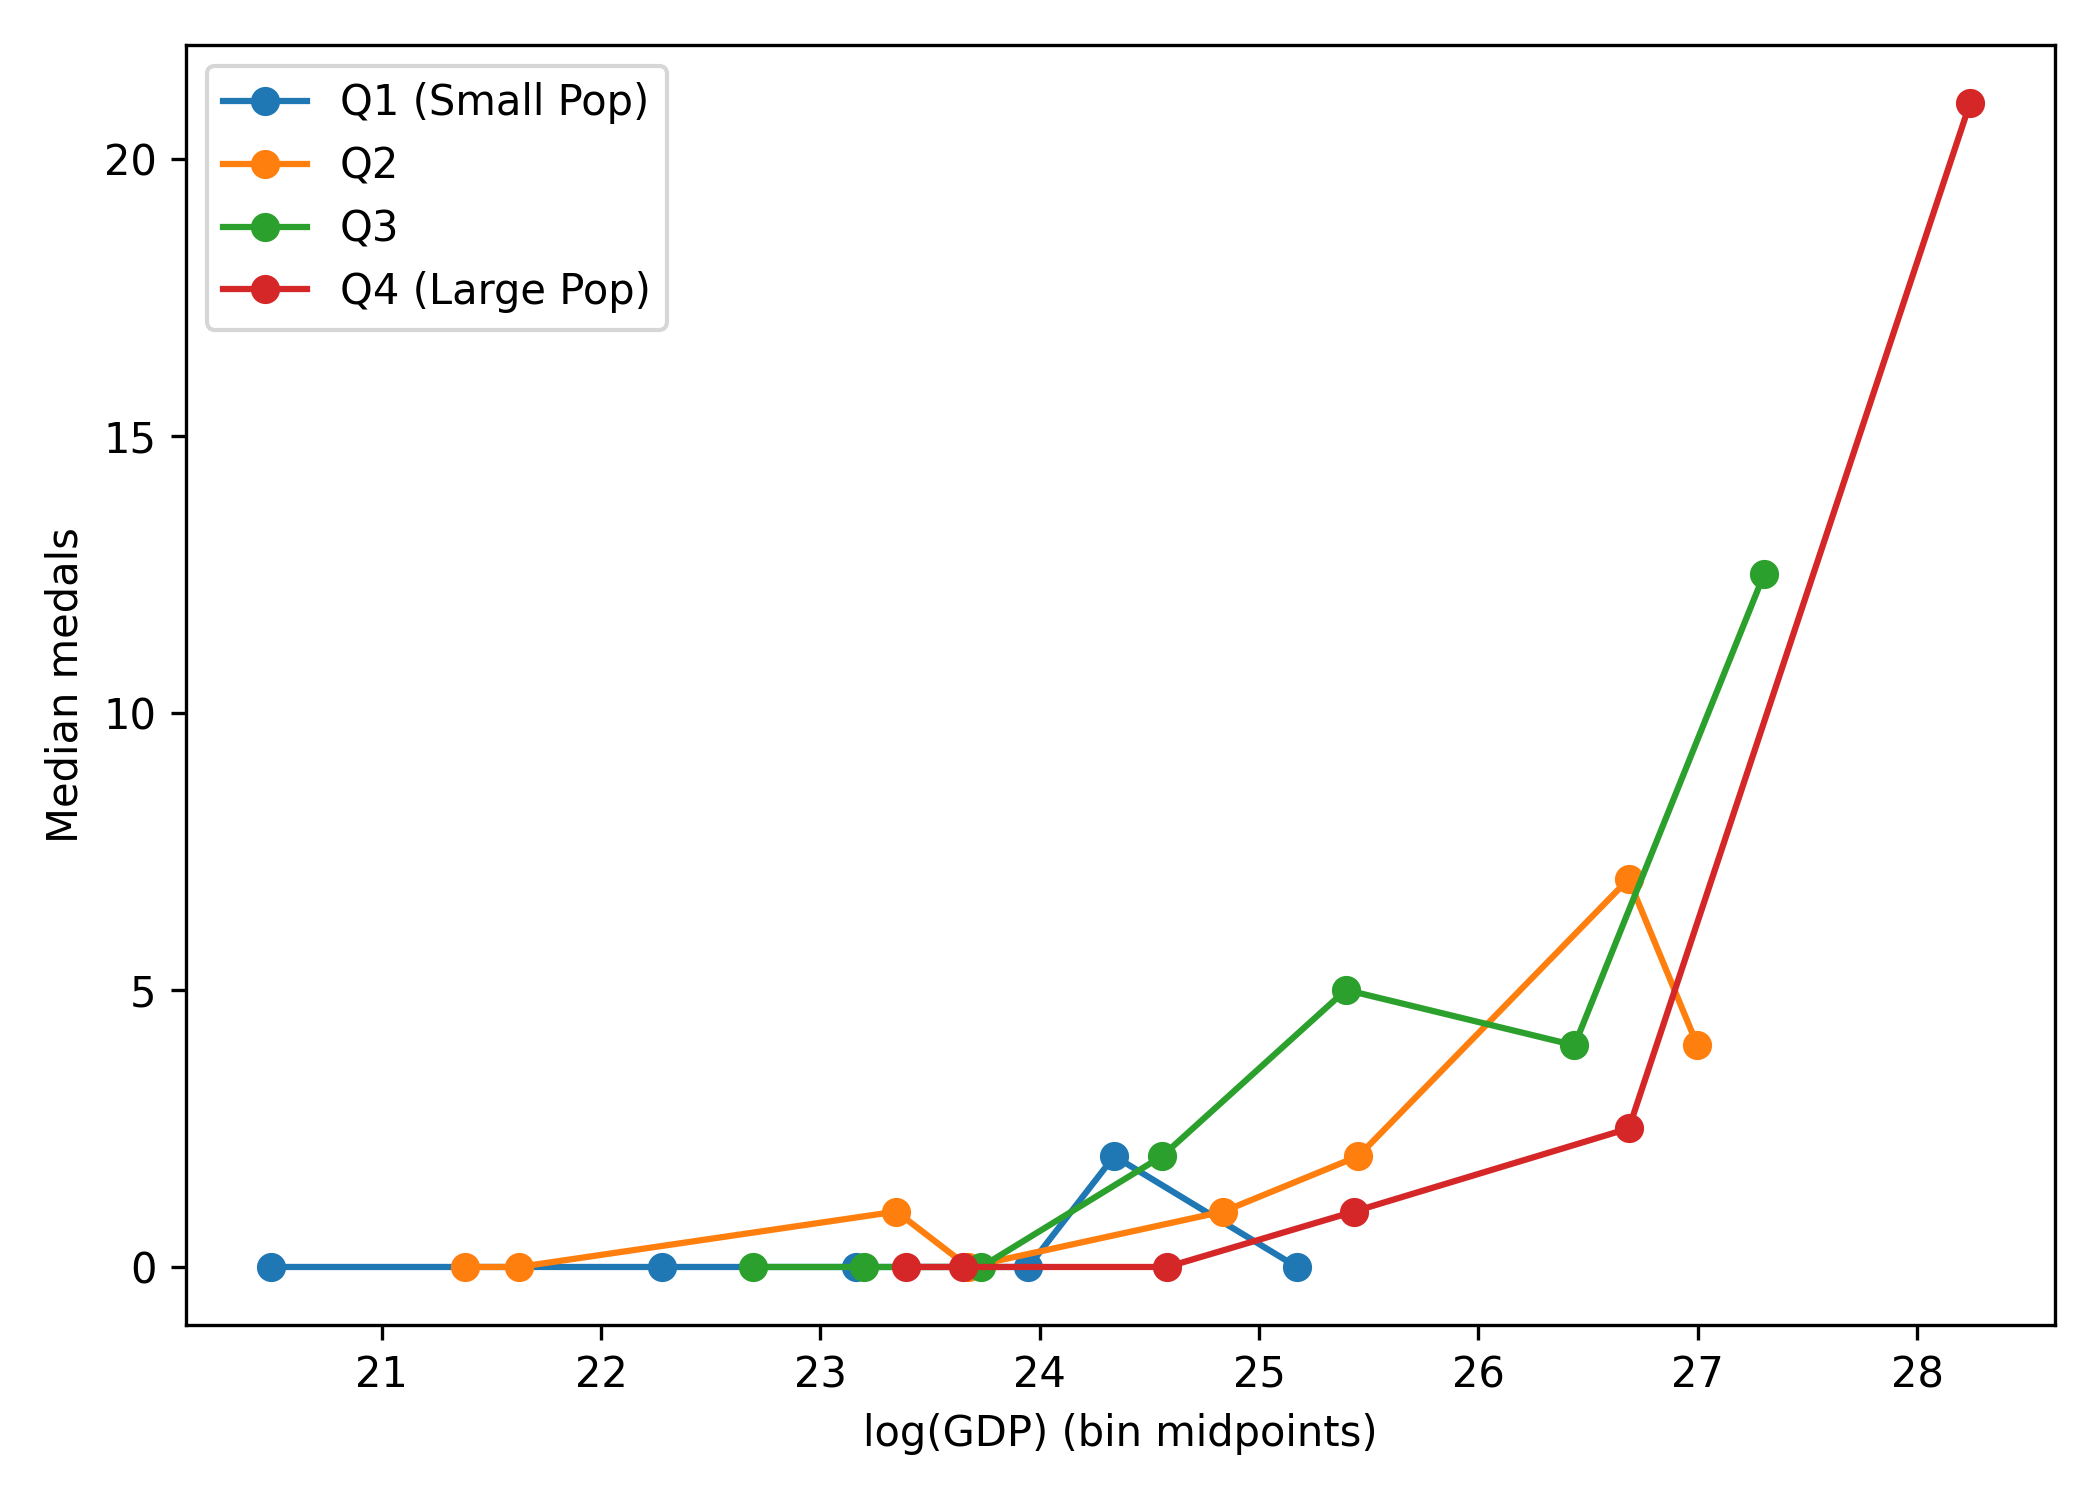
\includegraphics[width=0.75\textwidth]{fig_interaction_gdp_pop.png}
  \caption{Interaction pattern: GDP $\times$ Population (binned medians)}
  \label{fig:gdp_pop}
\end{figure}

Taken together, the figures corroborate the table-based findings: (i) interaction terms offer modest improvements in predictive accuracy (lower RMSE) with limited gains in parsimony (AIC/BIC); (ii) the \textbf{negative Athletes $\times$ HDI interaction} has clear substantive meaning—team expansion yields smaller marginal returns in high-HDI nations; and (iii) \textbf{GDP $\times$ Population} is negligible, indicating that medal counts are better explained by the main effects of economic size and population rather than their product. Consequently, we retain the baseline specification as the primary explanatory model and present interaction models as robustness checks.


% =============================================================================
% Conclusion
% =============================================================================
\section{Conclusion}

\subsection{Summary of Findings}
This study not only confirms the significant impact of national economic scale, population size, and the number of participating athletes on Olympic medal counts, but also provides a deeper understanding of the structural mechanisms behind Olympic success.  

First, the overall medal distribution reveals a persistent structural imbalance. Wealthy economies and large-population countries dominate the medal tables, whereas smaller or less-developed nations are more likely to remain in the “zero-medal” category. Such disparities are not incidental but rather the outcome of accumulated economic power, demographic resources, and long-term investment in sports development.  

Second, the positive effects of GDP and population go beyond the simple notion of “more money and more people.” They reflect broader advantages in sports infrastructure, technological support, and systematic training. The interaction between GDP and population underscores this effect: countries that are both wealthy and populous are almost inevitably positioned as Olympic powerhouses.  

Third, the number of athletes highlights the importance of opportunity structures. Delegation size is not only a direct indicator of resource allocation but also a precondition for medal competitiveness. Without sufficient athletes, even highly developed nations face limitations in medal output, regardless of their economic or social strength.  

Fourth, the Human Development Index (HDI), while weaker in its direct effect, becomes highly relevant when combined with athlete numbers. This interaction illustrates a “quality meets quantity” relationship: given similar delegation sizes, nations with higher HDI achieve greater medal efficiency. This demonstrates how long-term investments in education, healthcare, and social welfare indirectly translate into athletic performance.  

Overall, these findings demonstrate that Olympic success is not determined by a single factor, but rather by the interaction of multiple social, economic, and human capital conditions. The analysis reveals both the direct drivers of medal counts and the underlying structural inequalities in global sport.  

Finally, these findings carry broader implications for the Olympic Games. The unequal distribution of medals reflects not only sporting competition but also national development disparities. This conclusion resonates with previous research, while the present study provides stronger empirical confirmation by applying a Zero-Inflated Negative Binomial framework. In doing so, it advances both the methodological and substantive understanding of the global Olympic landscape.  

\subsection{Theoretical and Practical Contributions}
The study makes several theoretical contributions. First, it extends the methodological toolbox of sports economics by applying a ZINB framework that better accommodates zero-inflated and over-dispersed distributions compared to Poisson or negative binomial models. Second, it uncovers the complex interplay between economic, demographic, and developmental factors, offering a richer understanding of how national resources are translated into Olympic success. Third, by highlighting the role of interaction effects (GDP $\times$ Population, Athletes $\times$ HDI), the study expands upon previous literature that primarily focused on isolated single-variable effects.  

On the practical side, the findings offer important policy implications. They provide quantitative evidence for Olympic committees and policymakers, who can optimize delegation sizes and allocate resources more effectively based on economic and social contexts. Moreover, the results emphasize the significance of broader human development investments, such as education and healthcare, which indirectly enhance the competitiveness of athletes on the international stage. Particularly for developing countries, the findings suggest pathways to achieve competitiveness even with limited resources, while for advanced economies, they highlight the importance of maintaining balanced investment strategies without overconcentration in a few elite sports.  

\subsection{Policy Implications}
The findings carry meaningful policy implications. For developing countries, Olympic success is not solely determined by economic or demographic size but hinges on systematic support for athletes. Expanding delegation sizes and ensuring quality of participants requires long-term investment in infrastructure, grassroots sports development, and human capital formation. Policy measures should focus on broad-based development rather than short-term gains, enabling nations to translate demographic and economic growth into competitive advantage.  

For developed countries, while their economic and demographic advantages remain strong, the role of HDI underscores the importance of sustained investment in human development. Health, education, and welfare systems not only shape overall societal well-being but also provide a solid foundation for elite sports. Furthermore, the International Olympic Committee (IOC) and international sports federations should be mindful of the highly unequal distribution of medals. Overconcentration of success in a handful of nations risks undermining the Olympic ideal of inclusiveness. Policy measures such as capacity-building programs and financial assistance for less-developed countries could enhance diversity and representation in the Games.  

\subsection{Limitations}
Despite the valuable insights provided by this study, several limitations should be acknowledged. First, the measurement of Olympic success relies on the simple aggregation of gold, silver, and bronze medals. This approach overlooks the differences in competitive and symbolic value among the three medal types. In both official Olympic rankings and public perception, gold medals are often assigned greater importance, sometimes serving as the sole criterion for ranking. Consequently, treating all medal types as equal may underestimate the strength of countries with a high proportion of gold medals, while overestimating those whose success is concentrated in bronze medals. Nevertheless, the aggregated medal count remains one of the most widely used measures in the literature, providing a reasonable proxy for overall Olympic success.  

Second, although the explanatory variables in this study capture essential economic, demographic, and human capital factors, they do not fully reflect the broader mechanisms shaping Olympic outcomes. Elements such as national sports policies, historical traditions, cultural preferences, and host-country effects are also likely to influence medal distribution. Due to data availability and model complexity, these factors were not included, but their omission highlights potential avenues for future research.  

Finally, the analysis is based on a specific edition of the Olympic Games, which may limit the generalizability of the findings across other contexts.  

Despite these limitations, the findings of this study remain robust and credible. Rather than undermining the study’s contributions, these limitations highlight directions for further refinement and serve as a foundation for future investigations.  

\subsection{Future Research Directions}
Building on the limitations identified in this study, several promising directions for future research can be proposed.  

First, with regard to the measurement of Olympic success, future studies should move beyond the simple aggregation of gold, silver, and bronze medals. Developing weighted indices or composite indicators that account for the competitive and symbolic differences among medal types could provide a more nuanced and accurate assessment of national performance, mitigating the potential biases caused by treating all medals equally.  

Second, in terms of explanatory variables, future research could expand the analytical scope by integrating broader political, cultural, and institutional factors alongside economic, demographic, and human capital variables. National sports policies, cultural attitudes toward physical activity, historical sporting traditions, and host-country effects all represent potential determinants of Olympic outcomes. Interdisciplinary approaches drawing from sociology, political science, and cultural studies would help create a more comprehensive framework for understanding medal distribution.  

Third, regarding research scope and data, future studies could incorporate longitudinal datasets covering multiple editions of the Olympic Games. Such an approach would enhance the robustness and external validity of the findings while also enabling the exploration of dynamic trends in Olympic performance across different temporal and geographical contexts. Additionally, project-level or sport-specific data could shed light on how different events contribute to national medal success and resource allocation.  

In sum, future research that advances the measurement of success, broadens explanatory factors, and leverages longitudinal data will not only address the current study’s limitations but also contribute to a deeper and more systematic understanding of the determinants of Olympic achievements.  


% =============================================================================
% Bibliography
% =============================================================================
\bibliographystyle{abbrv}
\bibliography{literature}

\label{subsec:model_structure}

% =============================================================================
% Appendices
% =============================================================================
%\appendix
\appendix
\section*{Appendices}
\addcontentsline{toc}{section}{Appendices}

\section{Appendix 1}
\label{app:one}

The following script shows the essential steps for estimating the Zero-Inflated Negative Binomial (ZINB) model. 
It includes data preprocessing, model fitting, coefficient extraction, and generation of predictions. 
For full code (including extended diagnostics and plotting scripts), please refer to the GitHub repository.\footnote{\url{https://github.com/ZUTTER3150/Thesis-Draft-2}}

\begin{lstlisting}[caption={ZINB estimation on dataset1.xlsx using Python (statsmodels)}]
# ZINB on dataset1.xlsx 
# Mean model (count part):
#   log(u_i) = a + b*log(GDP_i) + c*log(Pop_i) + d*HDI_i + e*log(Athletes_i)
# Zero-inflation (inflation part): logit link, same set of covariates.
# Requirements: pip install pandas numpy statsmodels openpyxl

import numpy as np
import pandas as pd
import statsmodels.api as sm
from statsmodels.discrete.count_model import ZeroInflatedNegativeBinomialP

def to_numeric_clean(s: pd.Series) -> pd.Series:
    """Coerce to numeric safely: strip spaces, remove commas, set errors to NaN."""
    return pd.to_numeric(
        s.astype(str).str.strip().str.replace(",", "", regex=False),
        errors="coerce"
    )

# 1) Load & clean
file_path = "dataset1.xlsx"
df = pd.read_excel(file_path)

needed = ["Totalmedals", "GDP", "Population", "HDI", "Athletes"]
missing = [c for c in needed if c not in df.columns]
if missing:
    raise ValueError(f"Missing required columns: {missing}")

# Cast to numeric
for c in needed:
    df[c] = to_numeric_clean(df[c])

# Drop NAs
before = len(df)
df = df.dropna(subset=needed).copy()
print(f"[Info] Dropped {before - len(df)} rows with NA.")

# Require positive values for logs
for c in ["GDP", "Population", "Athletes"]:
    bad = (df[c] <= 0).sum()
    if bad:
        print(f"[Warn] {bad} rows non-positive {c}; removed.")
        df = df[df[c] > 0].copy()

# 2) Features 
df["log_GDP"] = np.log(df["GDP"])
df["log_Pop"] = np.log(df["Population"])
df["log_Athletes"] = np.log(df["Athletes"])

y = df["Totalmedals"].astype(int).values

# Count and inflation parts
X = sm.add_constant(df[["log_GDP", "log_Pop", "HDI", "log_Athletes"]])
Z = sm.add_constant(df[["log_GDP", "log_Pop", "HDI", "log_Athletes"]])

# 3) Fit ZINB
print("[Fit] ZINB with full inflation set...")
model = ZeroInflatedNegativeBinomialP(endog=y, exog=X, exog_infl=Z, inflation="logit")
res = model.fit(method="lbfgs", maxiter=600, disp=False)

print(res.summary())

# 4) Extract coefficients
coef = res.params
a = coef.get("const", np.nan)
b = coef.get("log_GDP", np.nan)
c = coef.get("log_Pop", np.nan)
d = coef.get("HDI", np.nan)
e = coef.get("log_Athletes", np.nan)

print("\n=== Count-part coefficients ===")
print(f"a = {a:.6f}, b = {b:.6f}, c = {c:.6f}, d = {d:.6f}, e = {e:.6f}")

# IRRs
irr = np.exp([a, b, c, d, e])
print("\nIRR (exp(coeff)):", irr)

# 5) Predictions and residuals
pi = res.predict(exog=X, exog_infl=Z, which="prob-zero")
mu = np.exp(a + b*df["log_GDP"] + c*df["log_Pop"] + d*df["HDI"] + e*df["log_Athletes"])
EY = (1.0 - pi) * mu

# Standardized residual
alpha_hat = float(coef.get("alpha", 0))
var_nb = mu + alpha_hat * (mu**2)
var_y = (1.0 - pi) * var_nb + pi * (1.0 - pi) * (mu**2)
std_resid = (y - EY) / np.sqrt(np.maximum(var_y, 1e-12))

out = pd.DataFrame({
    "Team": df.get("Team", pd.Series(index=df.index, dtype=object)),
    "Totalmedals": y,
    "E_total": EY,
    "std_resid": std_resid           
})
out.to_csv("zinb_predictions.csv", index=False)
print("[Saved] zinb_predictions.csv")

# 6) Plot partial effects (omitted for brevity)
# See full code for plotting functions and details.
\end{lstlisting}

\clearpage

\section{Appendix 2}
\label{app:two}
In addition to population, similar heterogeneity analyses were conducted by 
GDP, HDI, and the number of athletes. As the results and procedures are 
analogous across these dimensions, only the code for population grouping is 
presented here for illustration. The full scripts for all four categories can 
be accessed in the GitHub repository.\footnote{\url{https://github.com/ZUTTER3150/Thesis-Draft-2}}

The following script illustrates the computation of grouped residual statistics
by population size. Countries are divided into quartiles based on the logarithm 
of population size, and residuals (actual -- predicted medals) are summarized 
within each group.

\begin{lstlisting}[language=Python, caption={Grouped residuals by population size}, label={lst:pop_groups}]
import pandas as pd
import numpy as np
from pathlib import Path

# 1) Load predictions
PATH = Path("zinb_predictions.csv") 
df = pd.read_csv(PATH)

# 2) Residuals and population-size groups
df["residual"] = df["Totalmedals"] - df["E_total"]
labels = ["Small", "Medium-Small", "Medium-Large", "Large"]
df["Pop_group"] = pd.qcut(df["log_Pop"], q=4, labels=labels)

# 3) Grouped summary statistics
group_stats = (
    df.groupby("Pop_group", observed=True)
      .agg(
          n=("Team", "count"),
          mean_residual=("residual", "mean"),
          median_residual=("residual", "median"),
          sd_residual=("residual", "std"),
          mean_std_resid=("std_resid", "mean"),
          over_share=("residual", lambda x: np.mean(x > 0)),
          under_share=("residual", lambda x: np.mean(x < 0)),
      )
      .reset_index()
)

# 4) Save results
group_stats.to_csv("pop_groups_residuals.csv", index=False)
group_stats.to_latex(
    "pop_groups_residuals.tex",
    index=False, float_format="%.3f",
    caption="Prediction residuals by population-size groups (quartiles of log population).",
    label="tab:pop_groups_residuals"
)
\end{lstlisting}

\noindent\textbf{Notes:}
\begin{itemize}
    \item Residual = Actual $-$ Predicted; positive values indicate under-prediction.  
    \item ``Mean Std. Residual'' measures dispersion of standardized residuals.  
    \item ``Share Over-Perf.'' / ``Under-Perf.'' indicate the proportion of countries 
          with positive or negative residuals in each group.  
\end{itemize}

\clearpage

\section{Appendix 3}
\label{app:one}

For readability, only the core fitting and robustness-check code is shown below.  
Data preprocessing, diagnostics, and error-handling functions are available in the 
online repository.\footnote{\url{https://github.com/YourName/YourRepo}}  

\begin{lstlisting}[language=Python, caption={Core code for subsample robustness checks of ZINB and NB2 models}, label={lst:subsample_robustness}]
import pandas as pd
import numpy as np
import warnings
from statsmodels.discrete.count_model import (
    ZeroInflatedNegativeBinomialP, NegativeBinomialP
)
# 1) Define formulas
COUNT_FORMULA = "Totalmedals ~ log_GDP + log_Pop + HDI + log_Athletes"
INFL_FORMULA  = "~ log_GDP + log_Pop + HDI + log_Athletes"

# 2) Model fitting functions
def fit_zinb(data, label):
    """Fit ZINB model and return summary stats"""
    import patsy
    y, X = patsy.dmatrices(COUNT_FORMULA, data, return_type="dataframe")
    Z    = patsy.dmatrix(INFL_FORMULA, data, return_type="dataframe")

    model = ZeroInflatedNegativeBinomialP(
        endog=y, exog=X, exog_infl=Z,
        inflation="logit", p=2, maxiter=400
    )
    res = model.fit(disp=False, method="bfgs")
    return {"Subset": label, "Model": "ZINB", "LogLik": res.llf, "AIC": res.aic}

def fit_nb2(data, label):
    """Fit NB2 model and return summary stats"""
    import patsy
    y, X = patsy.dmatrices(COUNT_FORMULA, data, return_type="dataframe")
    model = NegativeBinomialP(endog=y, exog=X, p=2, maxiter=400)
    res = model.fit(disp=False, method="bfgs")
    return {"Subset": label, "Model": "NB2", "LogLik": res.llf, "AIC": res.aic}

# 3) Define subsamples
subsets = [
    ("Full sample", df.copy()),
    ("Drop top 3 medal countries",
        df[~df["Team"].isin(df.nlargest(3, "Totalmedals")["Team"])]),
    ("Drop small delegations",
        df[df["log_Athletes"] > df["log_Athletes"].quantile(0.25)]),
    ("Drop zero-medal nations",
        df[df["Totalmedals"] > 0]),
]

# 4) Run robustness checks
results = []
for label, dsub in subsets:
    try:
        row = fit_zinb(dsub, label)
    except Exception:
        row = fit_nb2(dsub, label)   # fallback if ZINB fails
    results.append(row)

summary = pd.DataFrame(results)
print(summary)
summary.to_latex("robustness_subsamples.tex", index=False)

\end{lstlisting}

\clearpage

\section{Appendix 4}
\label{app:one}


The following script tests sensitivity of the ZINB medal model to the inclusion of
interaction terms. Both baseline and extended specifications are fitted manually
with explicit design matrices. For clarity, only the essential code is reproduced
below; full diagnostics and robustness outputs are available in the GitHub 
repository.\footnote{\url{https://github.com/ZUTTER3150/Thesis-Draft-2}}

\begin{lstlisting}[language=Python, caption={ZINB model sensitivity with interaction terms}, label={lst:zinb_interaction_sensitivity}]
import pandas as pd
import numpy as np
import warnings
import statsmodels.api as sm
from statsmodels.discrete.count_model import ZeroInflatedNegativeBinomialP

# 1) Load and clean data
df = pd.read_csv("zinb_predictions.csv")
df = df[["Team","Totalmedals","log_GDP","log_Pop","HDI","log_Athletes"]].dropna()
df["Totalmedals"] = df["Totalmedals"].clip(lower=0).round().astype(int)

# Center predictors and build interactions
for v in ["log_GDP","log_Pop","log_Athletes","HDI"]:
    df[f"c_{v}"] = df[v] - df[v].mean()
df["int_GDPxPop"] = df["c_log_GDP"] * df["c_log_Pop"]
df["int_AthxHDI"] = df["c_log_Athletes"] * df["c_HDI"]

# 2) ZINB fitting helper
def fit_zinb_manual(data, count_vars, infl_vars, label):
    y = data["Totalmedals"].values
    X = sm.add_constant(data[count_vars], has_constant="add")
    Z = sm.add_constant(data[infl_vars], has_constant="add")
    Z = Z.rename(columns={"const":"inflate_const"})
    model = ZeroInflatedNegativeBinomialP(endog=y, exog=X, exog_infl=Z,
                                          inflation="logit", p=2, maxiter=500)
    res = model.fit(disp=False, method="bfgs")
    return res

def collect_stats(label, res, Xcols):
    mu = res.predict(which="mean")
    rmse = float(np.sqrt(np.mean((df["Totalmedals"] - mu)**2)))
    params = res.params
    out = {"Model": label, "LogLik": res.llf,
           "AIC": res.aic, "BIC": res.bic,
           "RMSE": rmse, "alpha": params.get("alpha", np.nan)}
    return out

# 3) Specifications and runs
base_vars = ["log_GDP","log_Pop","HDI","log_Athletes"]
specs = [
    ("Baseline", base_vars, base_vars),
    ("Add GDPxPop", base_vars+["int_GDPxPop"], base_vars),
    ("Add AthletesxHDI", base_vars+["int_AthxHDI"], base_vars),
    ("Add both", base_vars+["int_GDPxPop","int_AthxHDI"], base_vars),
]

rows = []
for label, cvars, ivars in specs:
    res = fit_zinb_manual(df, cvars, ivars, label)
    rows.append(collect_stats(label, res, cvars))

cmp = pd.DataFrame(rows).sort_values("AIC")
print(cmp)
cmp.to_latex("zinb_interactions_comparison.tex", index=False)
\end{lstlisting}

\clearpage

\end{document}

